\documentclass[aspectratio=169, compress]{beamer}

\usepackage[T1]{fontenc}
\usepackage[utf8]{inputenc}
\usepackage[english]{babel}
\usepackage{animate}
\usepackage{pgfplots}
\pgfplotsset{compat=newest}
\usepackage{booktabs}
\usepackage{siunitx}
\usepackage{subcaption}
\usepackage{tikz}
\usepackage{tikz-3dplot}
\usepackage{bm}
\usetikzlibrary{calc}
\usepackage{tikzpagenodes}
\usepackage{amsmath,amssymb,amsfonts, stmaryrd}
\usepackage{pgfplots}
\usetikzlibrary{shapes,arrows,decorations.pathmorphing,backgrounds,positioning,fit,matrix}
\usepackage{mathtools} %Fixes/improves amsmath
\usepackage{lipsum}
\pgfplotsset{compat=1.8}
\usepackage{graphics} % for pdf, bitmapped graphics files
\usepackage{epsfig} % for postscript graphics files
\usetikzlibrary{spy}
% Latin Modern
\usepackage{lmodern}
% Verdana font type
%\usepackage{verdana}
% Helvetica
%\usepackage{helvet}
% Times (text and math)
%\usepackage{newtx, newtxmath}
% Nice font combination
%\usepackage{mathptmx} % math
%\usepackage{sourcesanspro} % sans-serif
\usepackage{charter} % serif

\usetheme[department=compute]{DTU}
%\useoutertheme[subsection=false]{miniframes}
%\useoutertheme{split}
\setbeamercovered{transparent}
%\setcounter{currentslide}{\the\beamer@slideinframe}

\title[Advanced Image Analysis 2019]{Assignment: Blob detection \& Feature Based Image Analysis}
\author{Xiao Hu$^1$}
\institute{$^1$: Technical University of Denmark}
\date{\today}

\newcommand{\tabitem}{{\color{dtured}$\bullet$} }

\begin{document}
	\frame{
		\maketitle
	}
	
%	\frame{
%		%\frametitle{Outline}
%		%\tableofcontents
%	}
	
	
	
	\section{Blob Detection}
	\subsection{Results}
	\frame{
		\frametitle{Scale-Space Blob Detection}
		\begin{columns}
			\column{.3\textwidth}
			Detailed steps :
			\begin{itemize}
				\item Localize blobs' center: Gaussian smoothing ($1$D kernel two times along $x$ \& $y$) and find local maxima (image dilate).
				\item Compute normalized Laplacian and find the minimum over scales at detected blobs' center.
			\end{itemize}

			\column{.6\textwidth}
			\begin{figure}
				\centering
				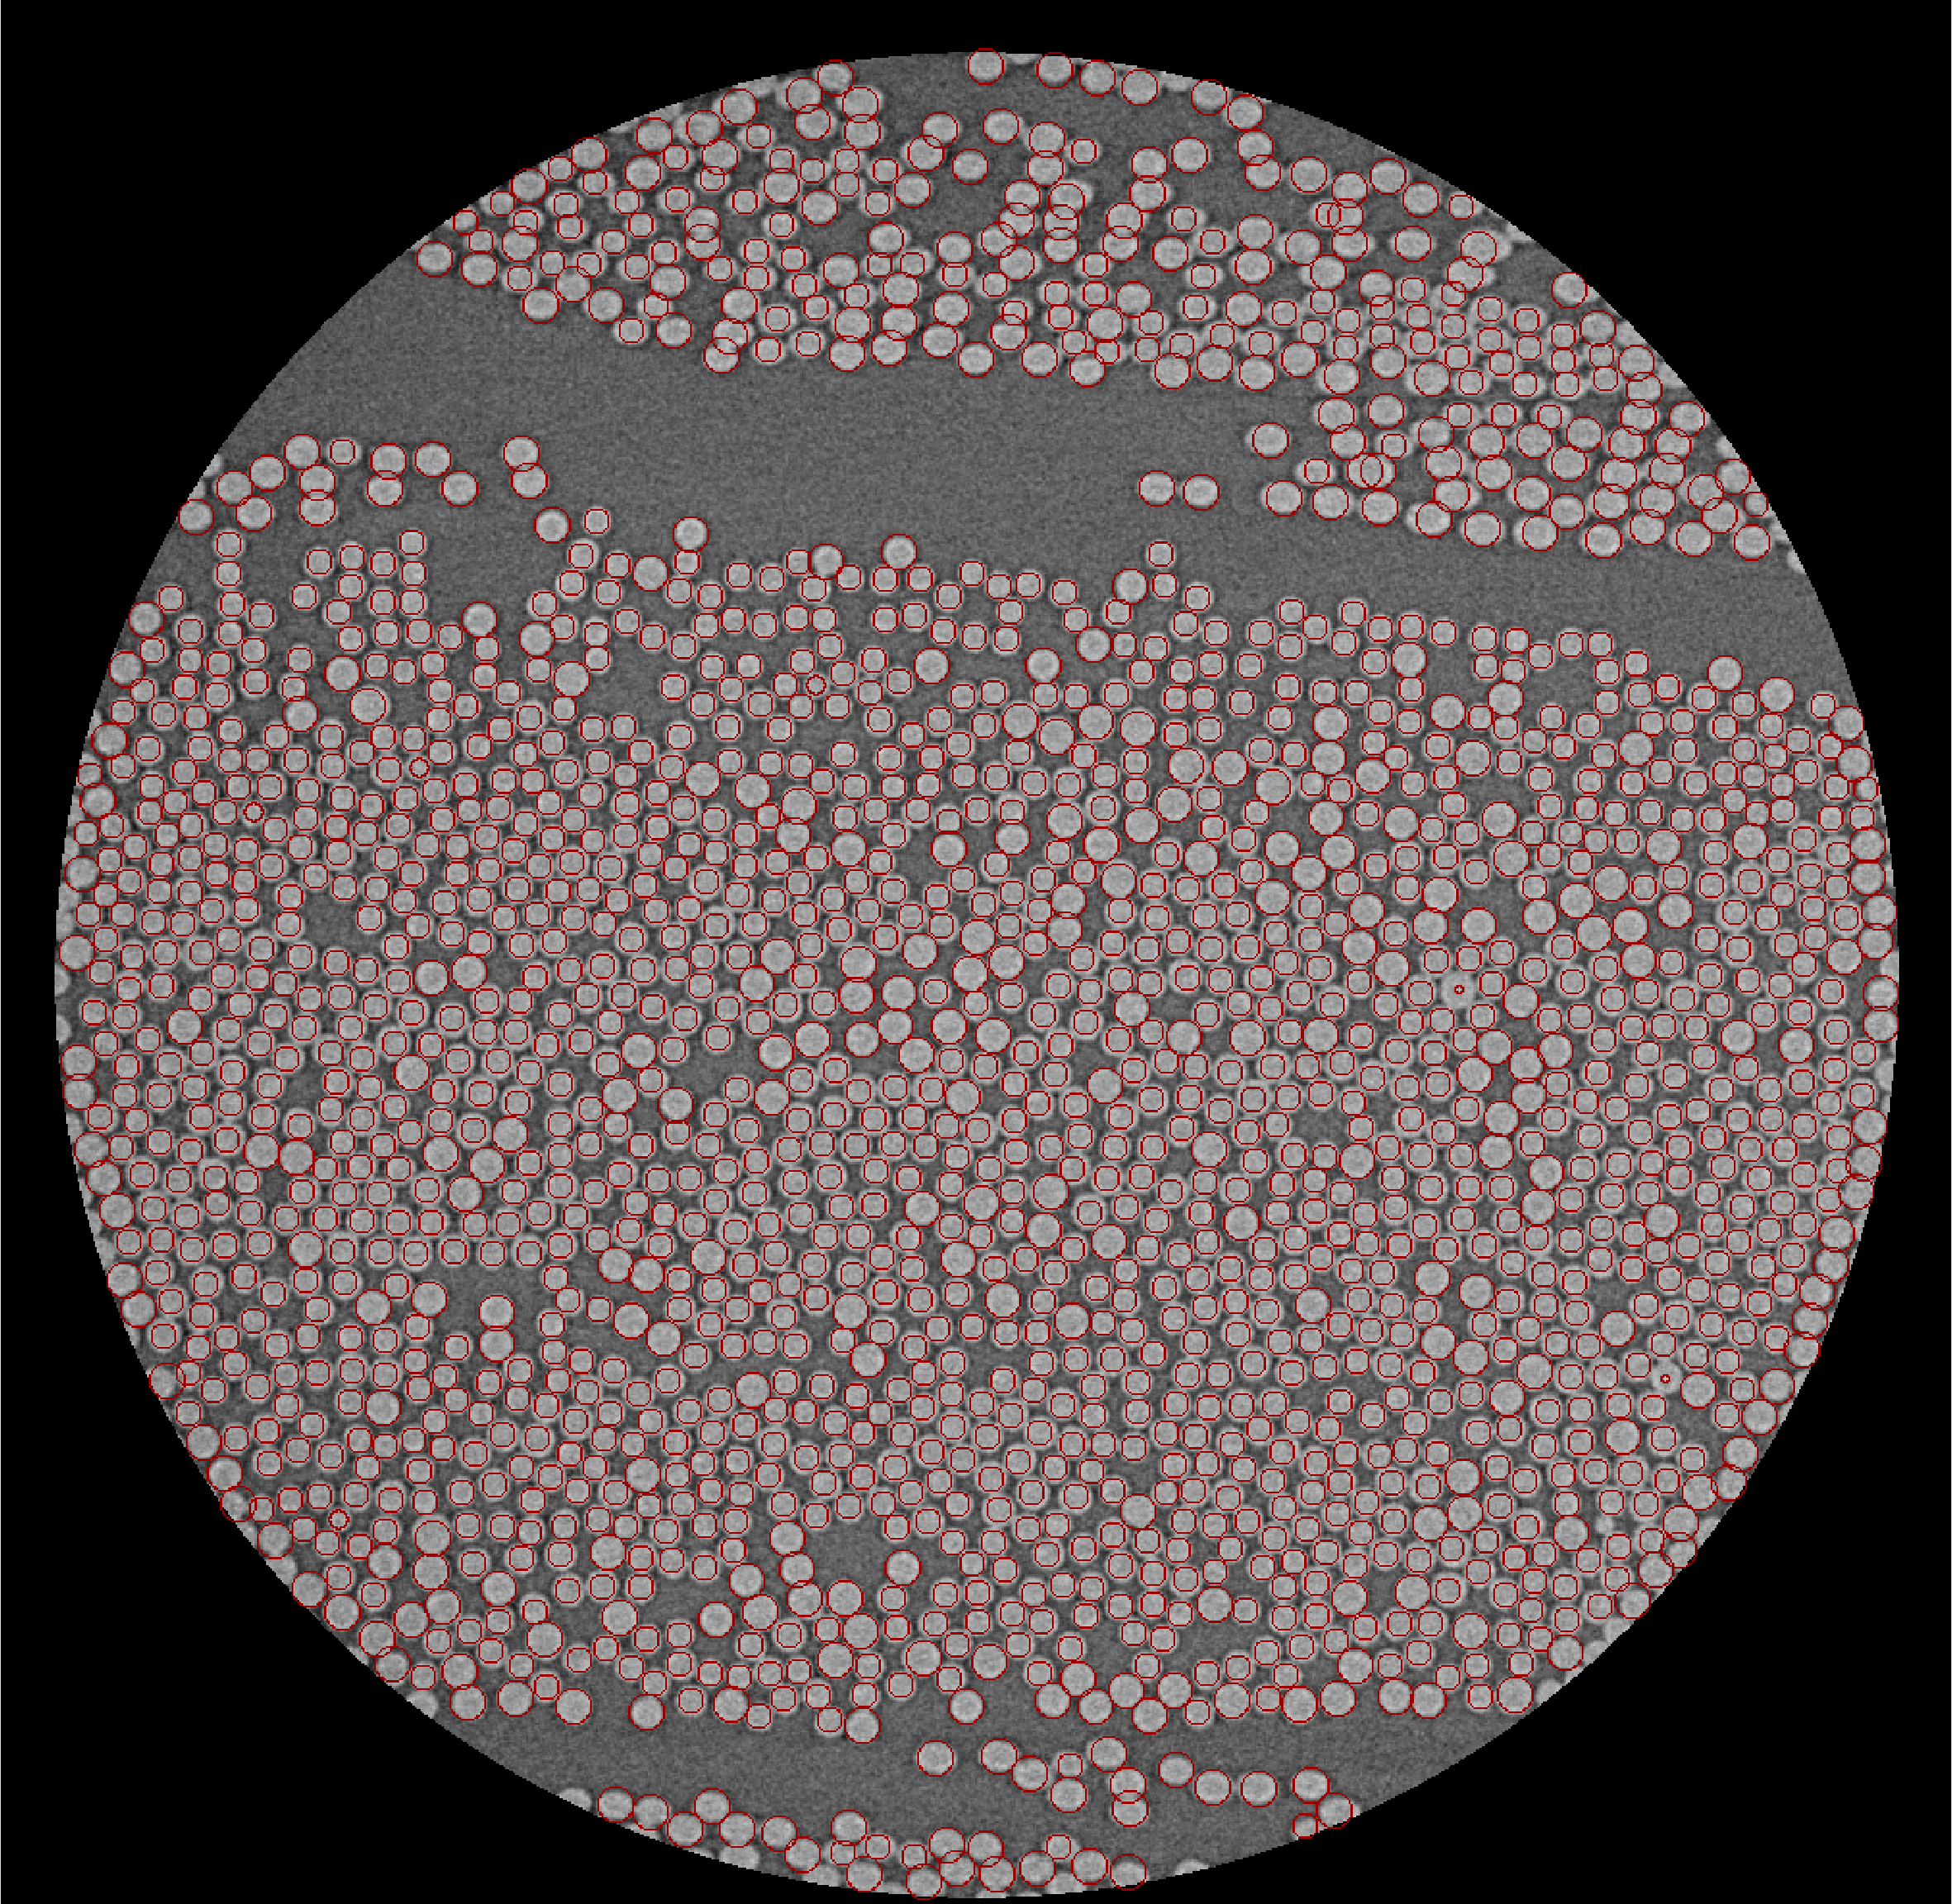
\includegraphics[width=0.65\textwidth]{figures/ex21.png}
				\caption{Result of \textit{CT\_lab\_high\_res.png}.}
			\end{figure}
		\end{columns}
	}
	\frame{
		\frametitle{Scale-Space Blob Detection}
			\begin{minipage}{.49\textwidth}
					\begin{figure}
					\centering
					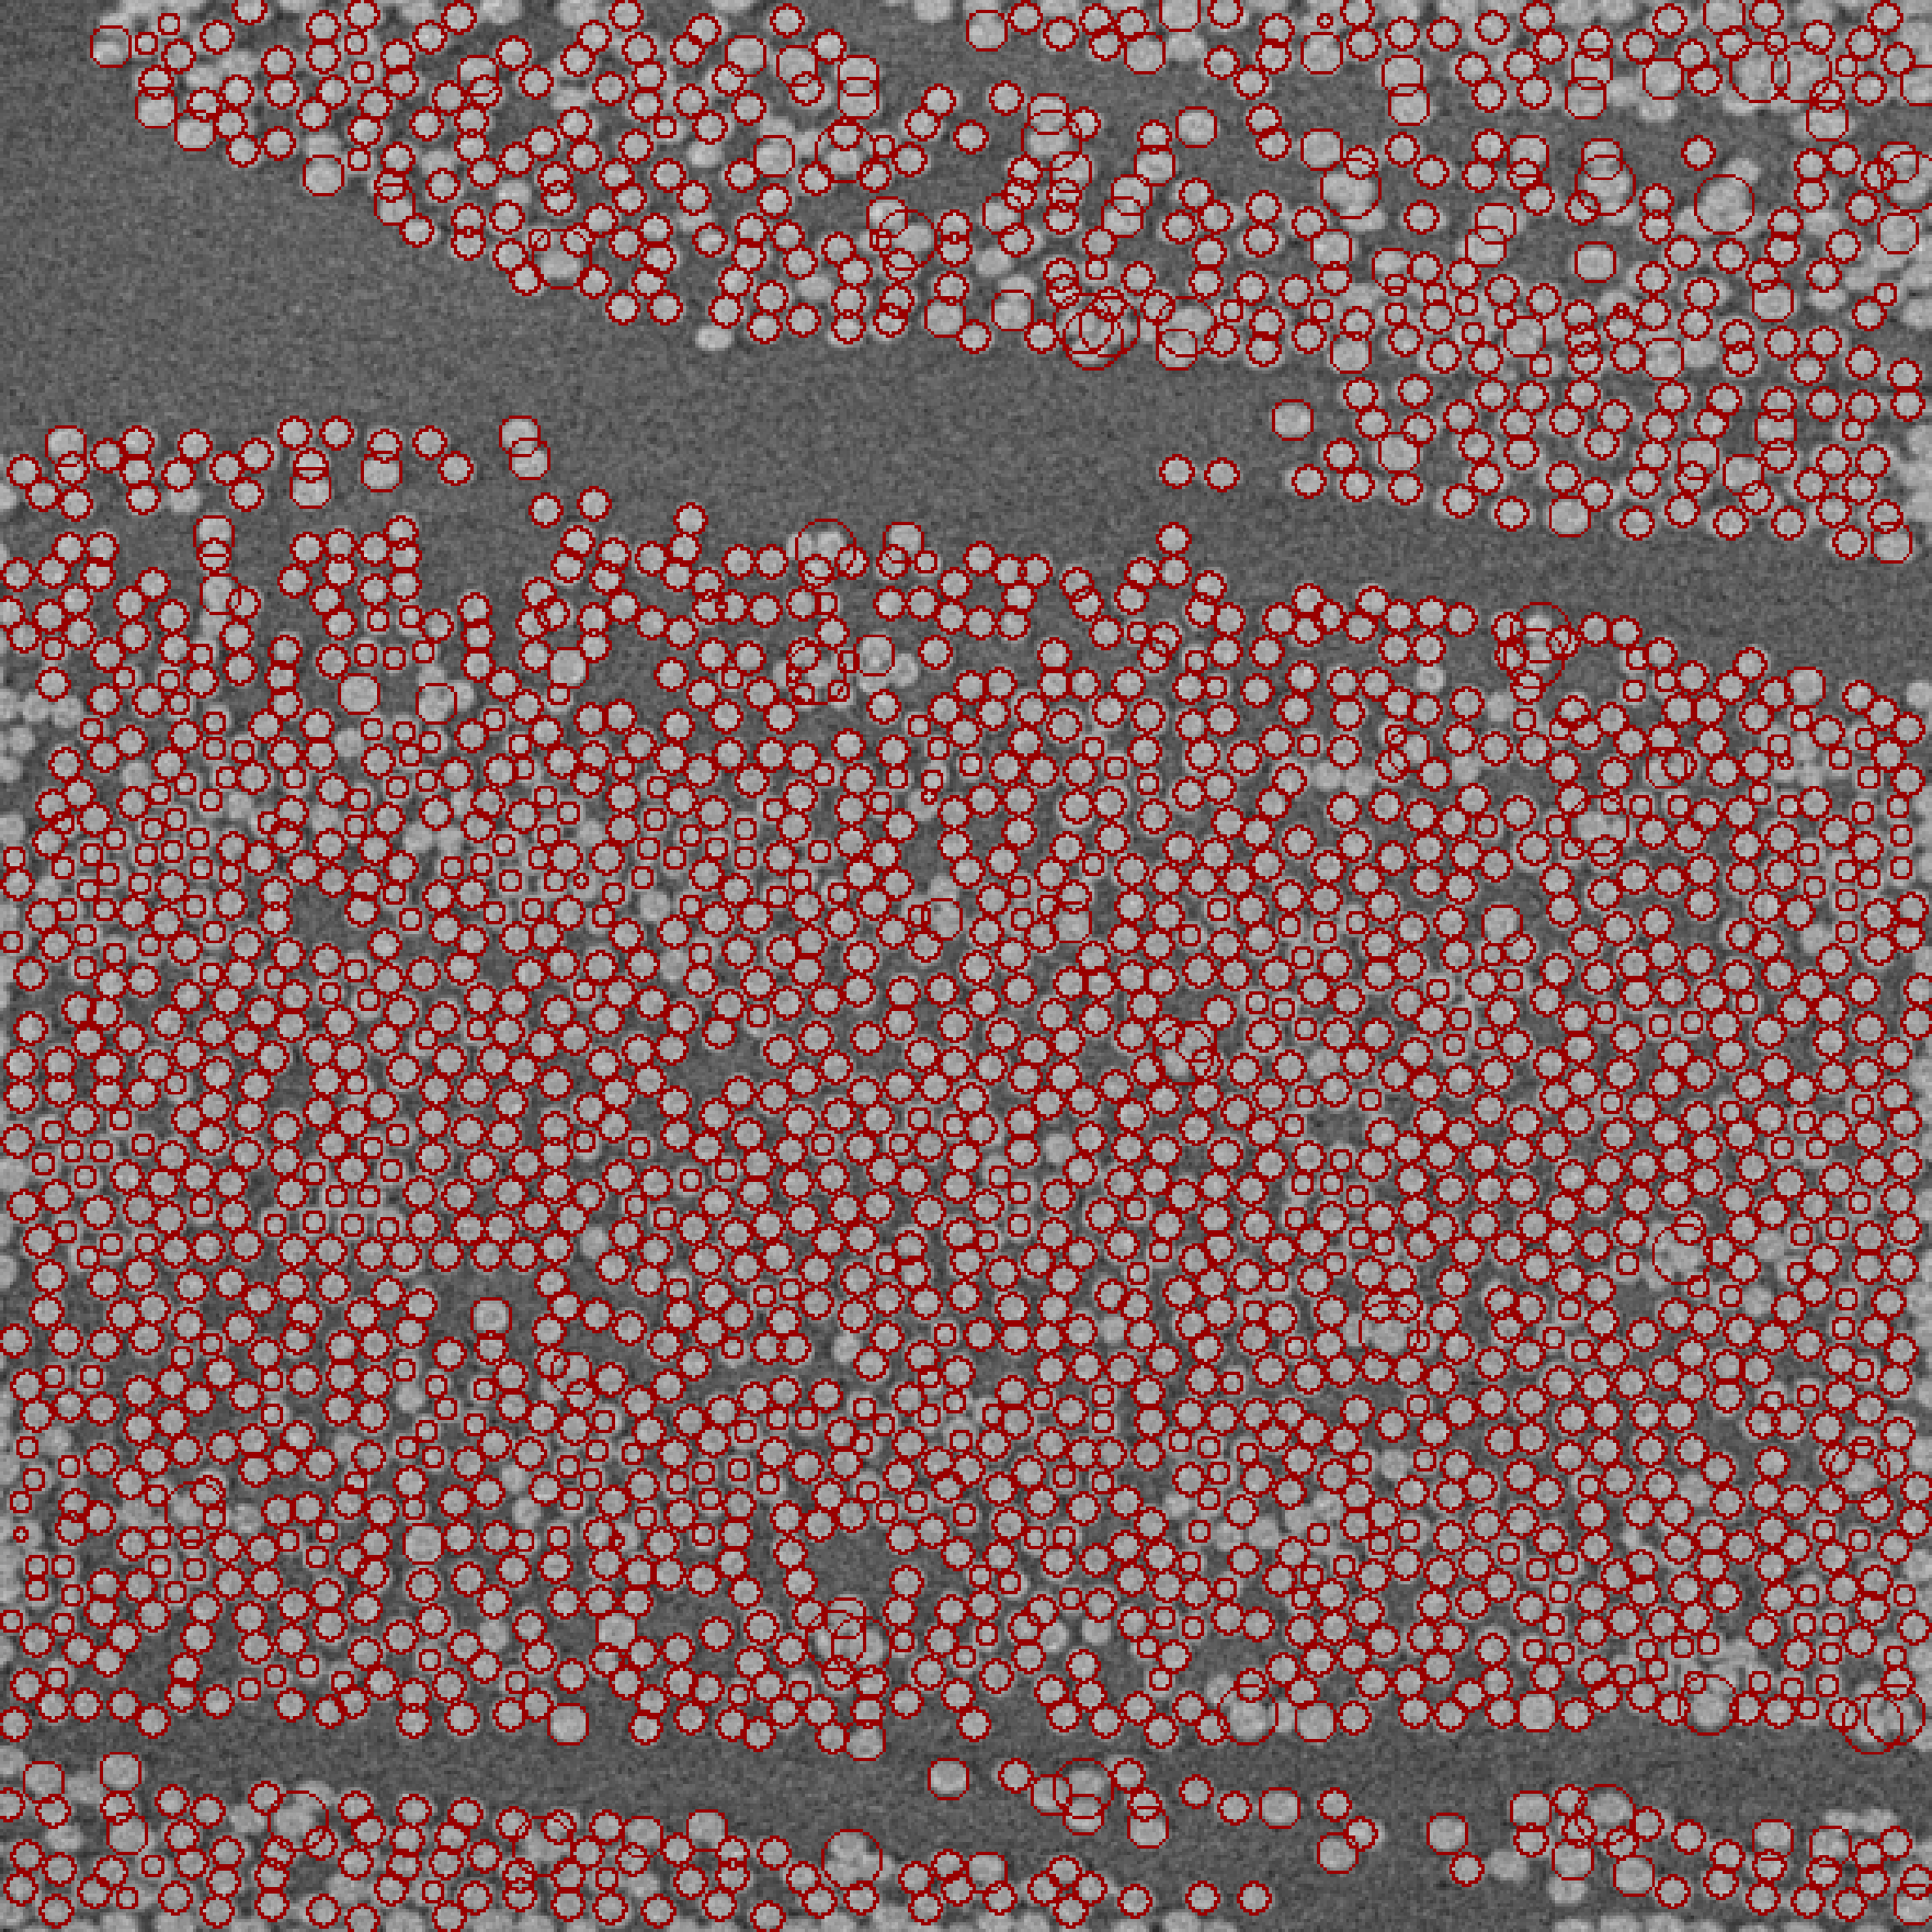
\includegraphics[width=0.8\textwidth]{figures/ex22.png} 
					\caption{Result of \textit{CT\_lab\_med\_res.png}.}
					\end{figure}
				\end{minipage}
				\begin{minipage}{.49\textwidth}
				\begin{figure}
					\centering
					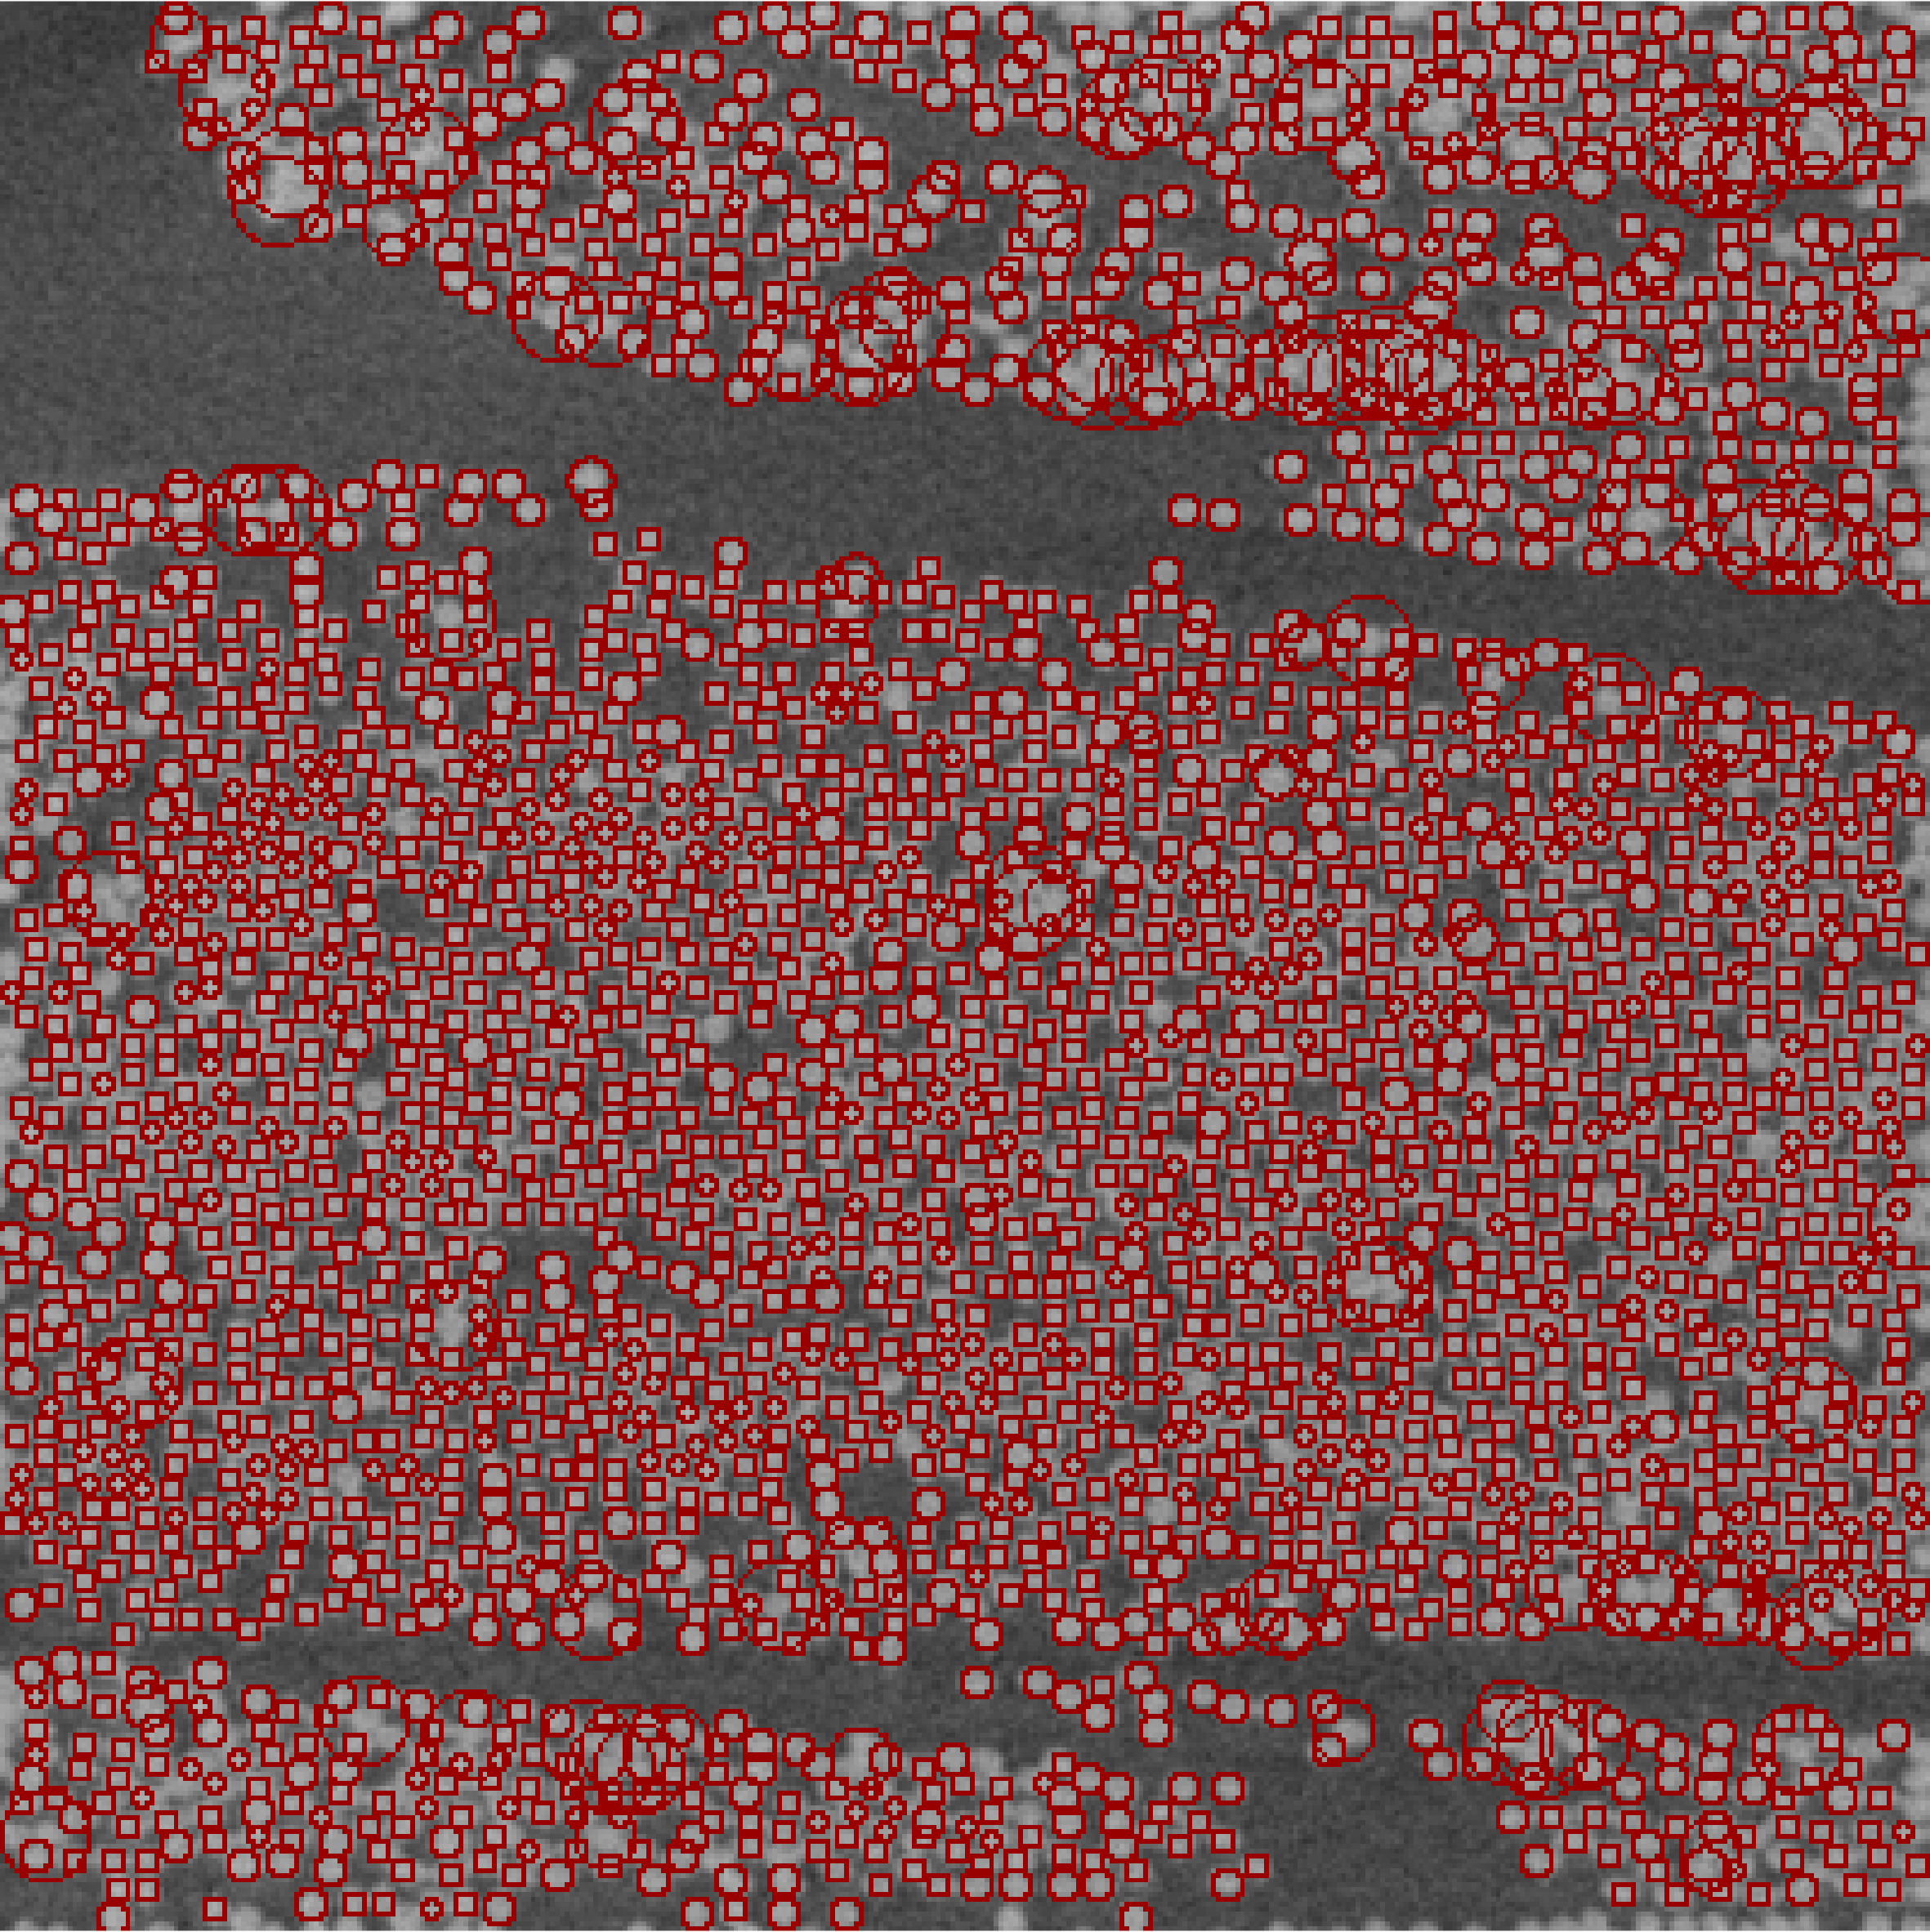
\includegraphics[width=0.8\textwidth]{figures/ex23.png}
					\caption{Result of \textit{CT\_lab\_low\_res.png}.}
				\end{figure}
				\end{minipage}
		}
	\frame{
		\frametitle{Scale-Space Blob Detection}
			\begin{minipage}{.49\textwidth}
					\begin{figure}
					\centering
					\includegraphics[width=0.8\textwidth]{figures/ex24.png} 
					\caption{Result of \textit{CT\_synchrotron.png}.}
					\end{figure}
				\end{minipage}
				\begin{minipage}{.49\textwidth}
				\begin{figure}
					\centering
					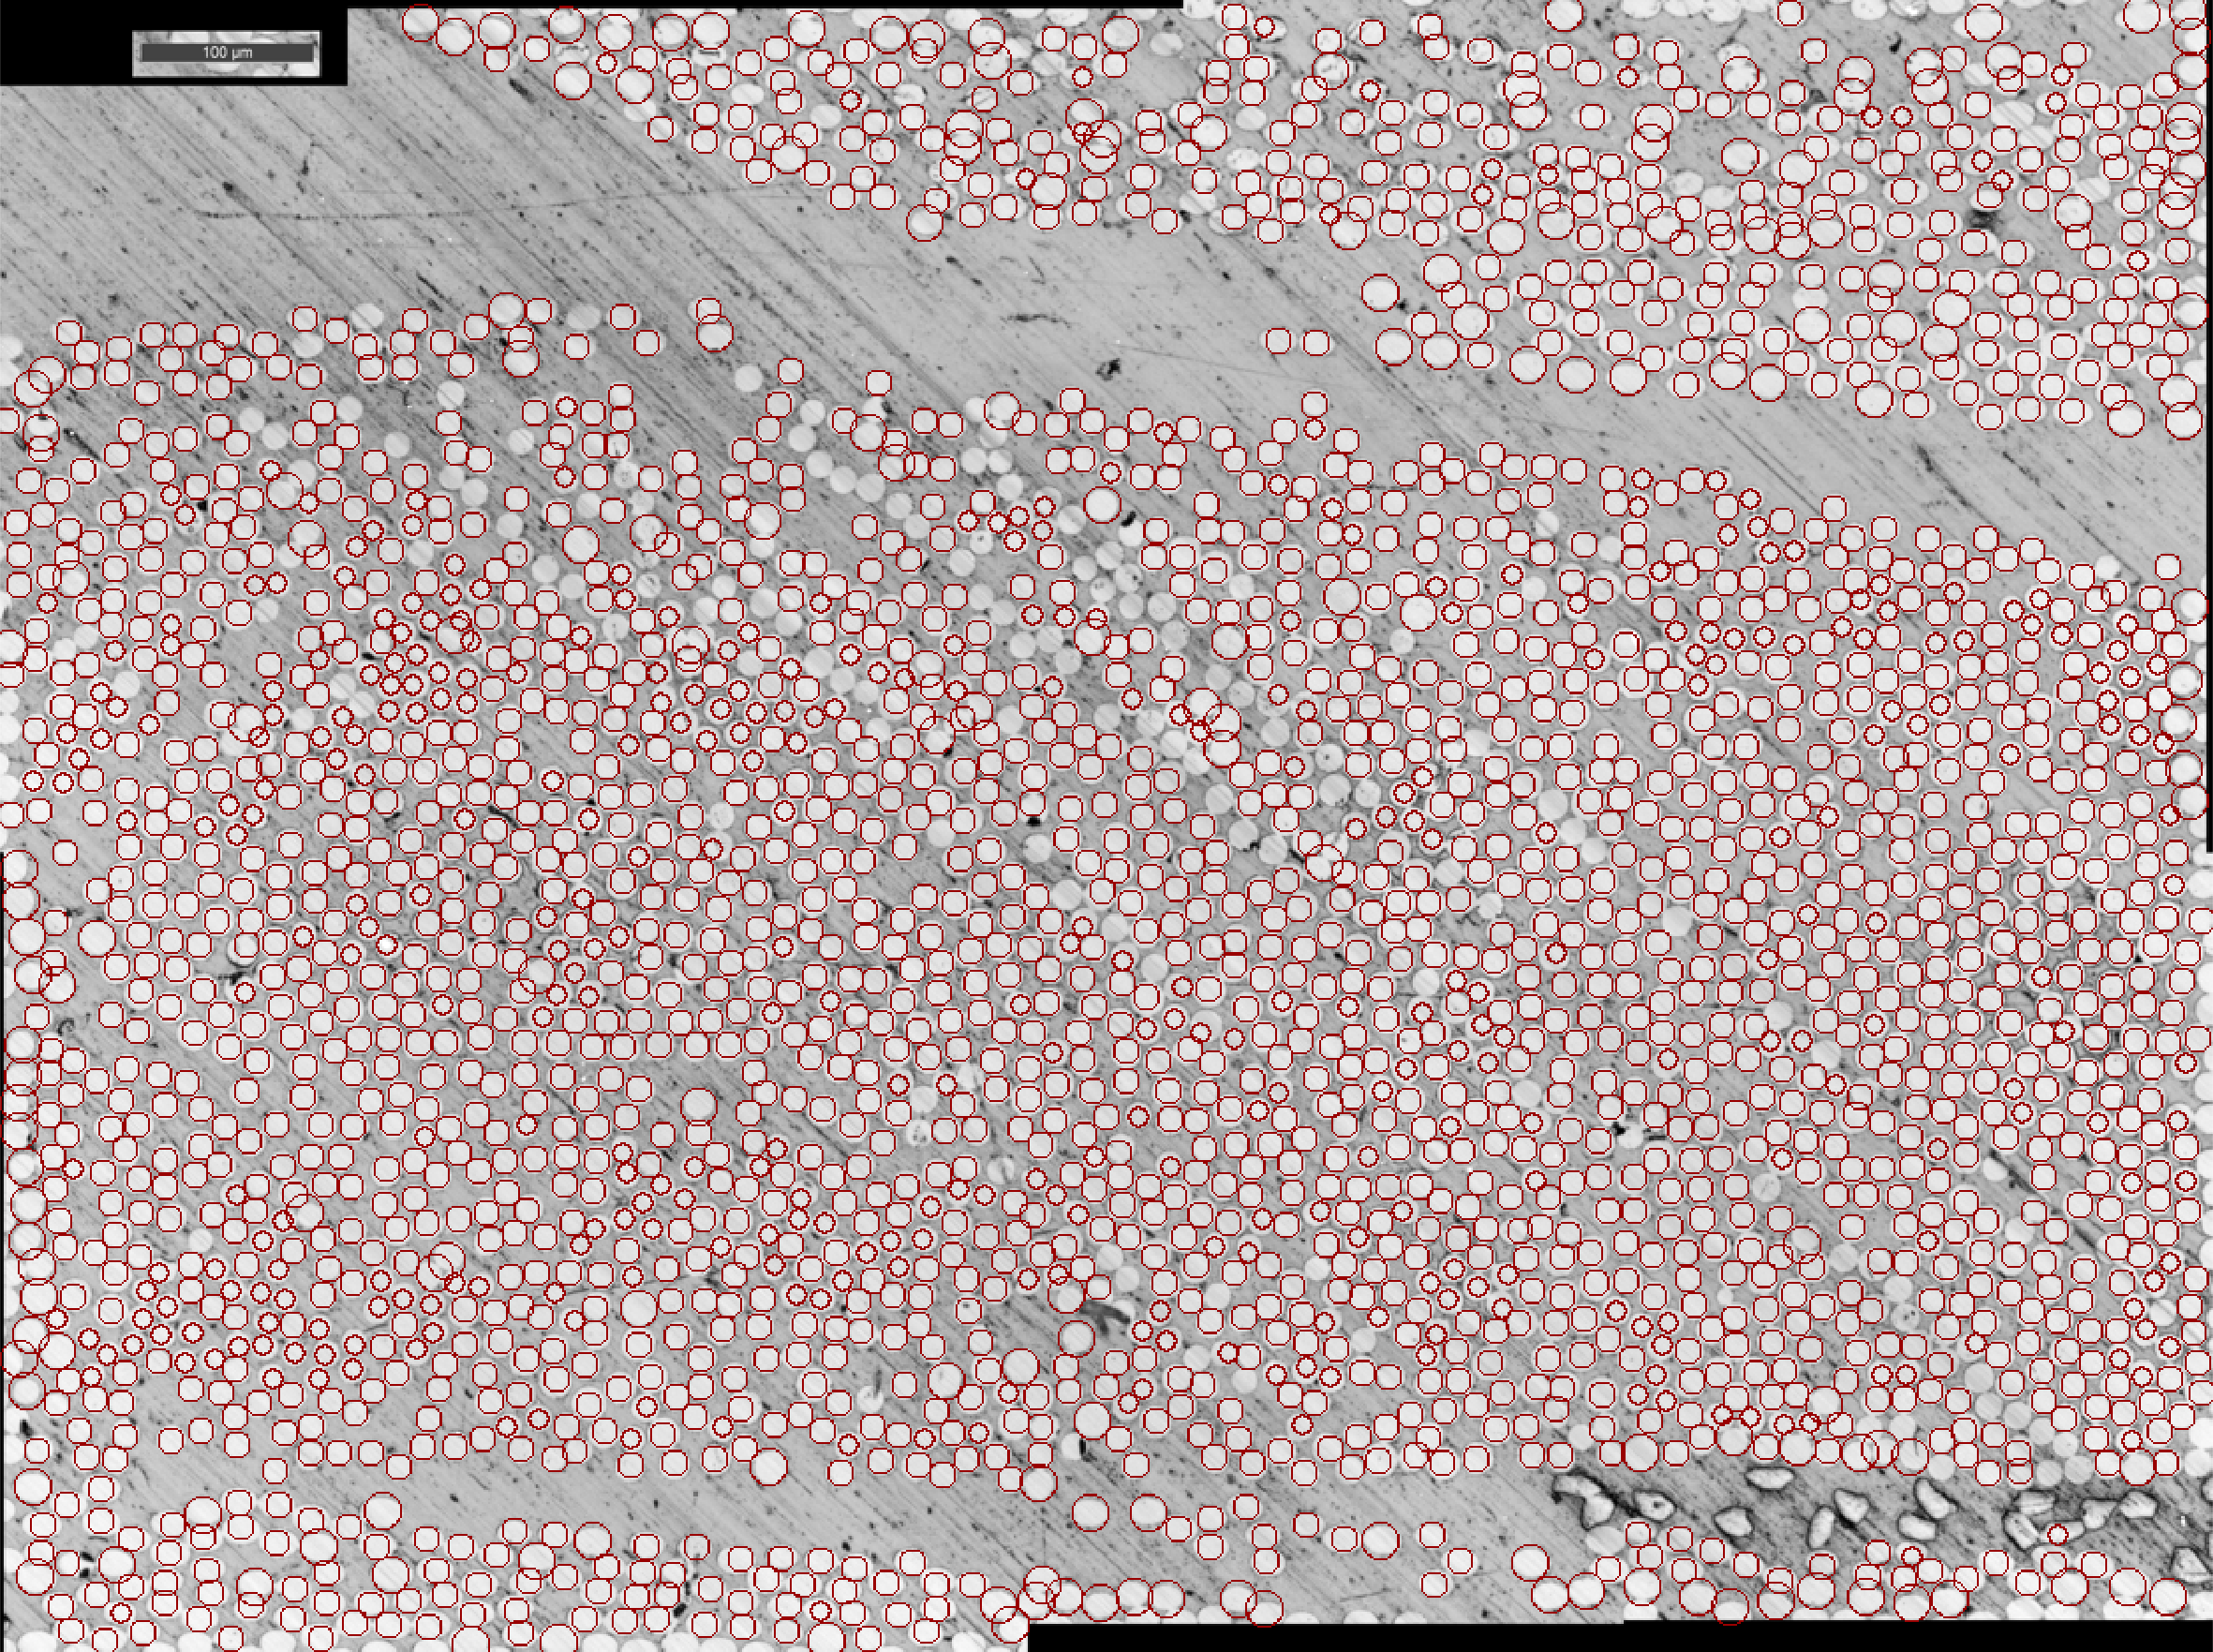
\includegraphics[width=0.9\textwidth]{figures/ex25.png}
					\caption{Result of \textit{Optical.png}.}
				\end{figure}
				\end{minipage}
		}		
	\frame{
		\frametitle{Scale-Space Blob Detection}
			\begin{minipage}{.9\textwidth}
					\begin{figure}
					\centering
					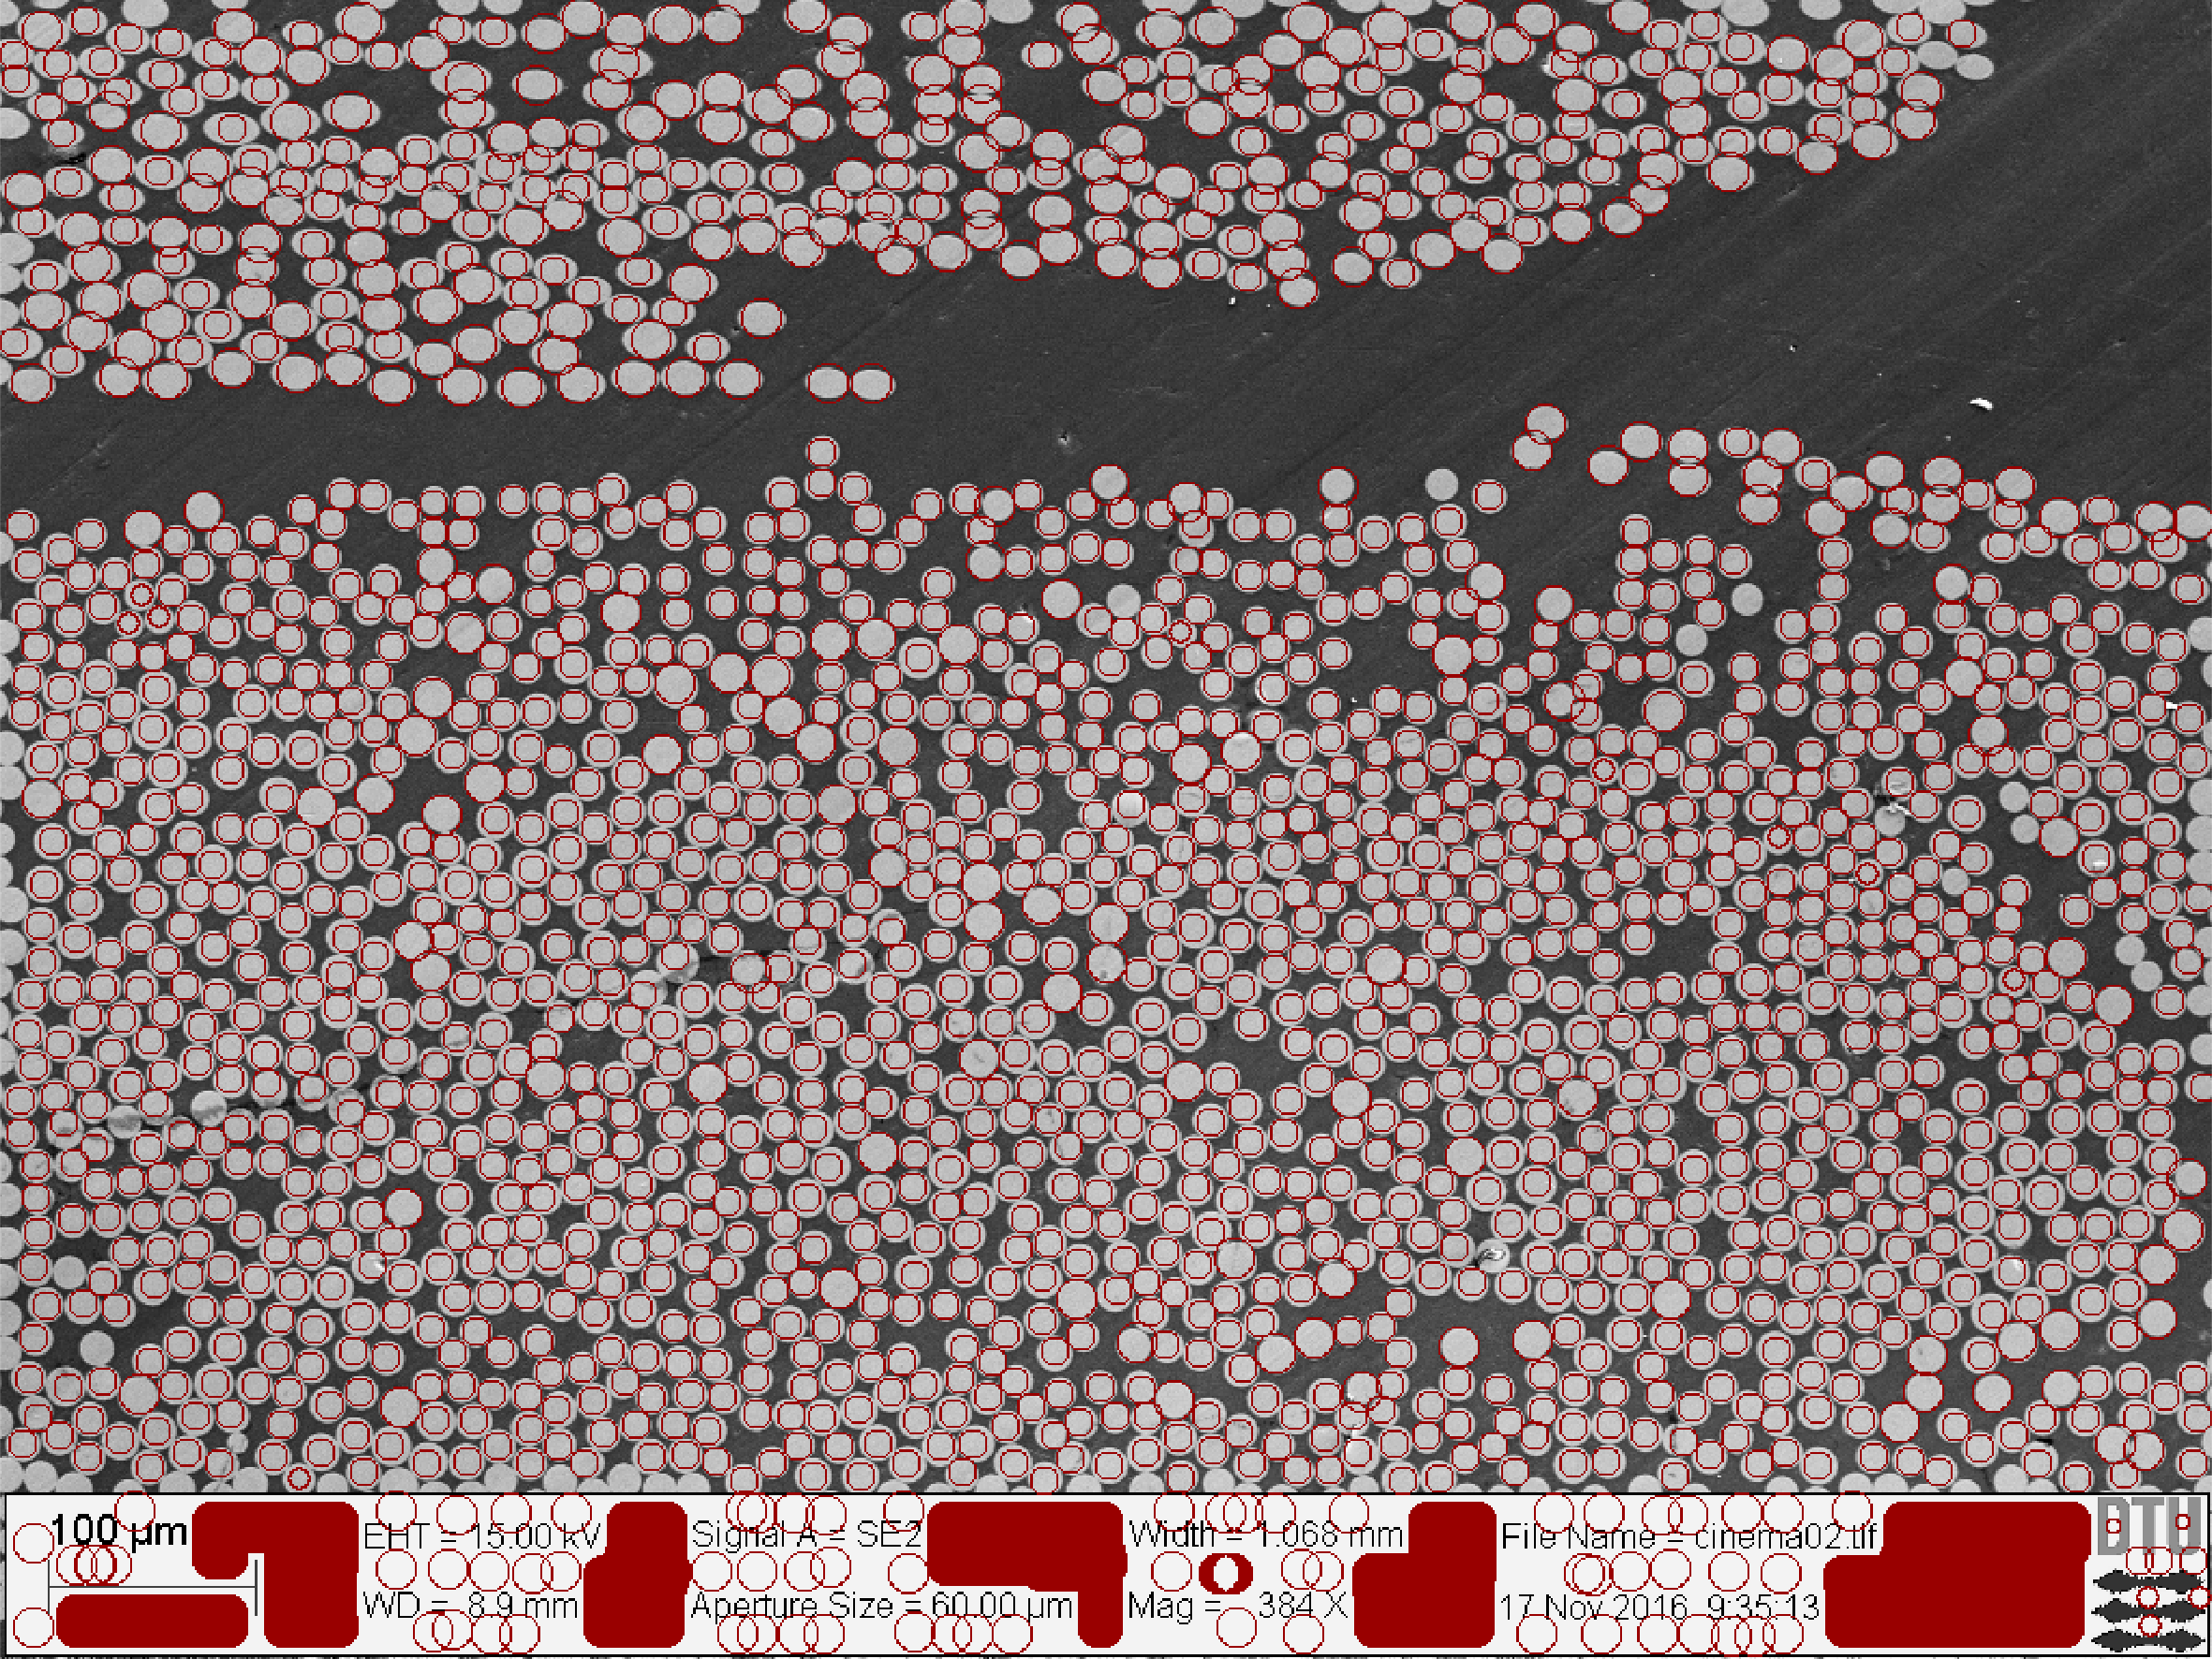
\includegraphics[width=0.6\textwidth]{figures/ex26.png} 
					\caption{Result of \textit{SEM.png}.}
					\end{figure}
				\end{minipage}
		}				
	\section{Feature Based Analysis}
	\subsection{Results}
	\frame{
		\subsection{Estimate $2$D Similarity Transformation}
		\frametitle{Estimate $2$D Similarity Transformation}
		Given $2$ sets ($\mathbf{p,q}$) of $2$D points with known correspondence, estimate $\mathbf{R,t},s$ which optimally aligns these two sets:
		\begin{enumerate}
		\item compute centroids: $\mu_{p}=\frac{1}{n}\sum_{i=1}^{n}\mathbf{p}_i$ and $\mu_{q}=\frac{1}{n}\sum_{i=1}^{n}\mathbf{q}_i$
		\item estimate scale: $s=\frac{\sum_{i=1}^{n}||\mathbf{q}_i-\mu_{q}||}{\sum_{i=1}^{n}||\mathbf{p}_i-\mu_{p}||}$
		\item Re-scaling $\mathbf{q}_i=\mathbf{q}_i/s$ and $\mu_{q}=\mu_{q}/s$, then compute $\mathbf{C}=\sum_{i=1}^{n}(\mathbf{q}_i-\mu_{q})(\mathbf{p}_i-\mu_{p})^T$
		\item $[\mathbf{U,S,V}]=svd(\mathbf{C})$, then $\mathbf{R}=\mathbf{U}\left[\begin{matrix} 1 & 0 \\ 0 & det(\mathbf{U}\mathbf{V}^T)\end{matrix}\right]\mathbf{V}^T$
		\item $\mathbf{t}=\mu_{q}-\mathbf{R}*\mu_{p}$
		\end{enumerate}
	}
	\frame{
		\frametitle{Estimate $2$D Similarity Transformation}
			\begin{minipage}{.49\textwidth}
					\begin{figure}
					\centering
					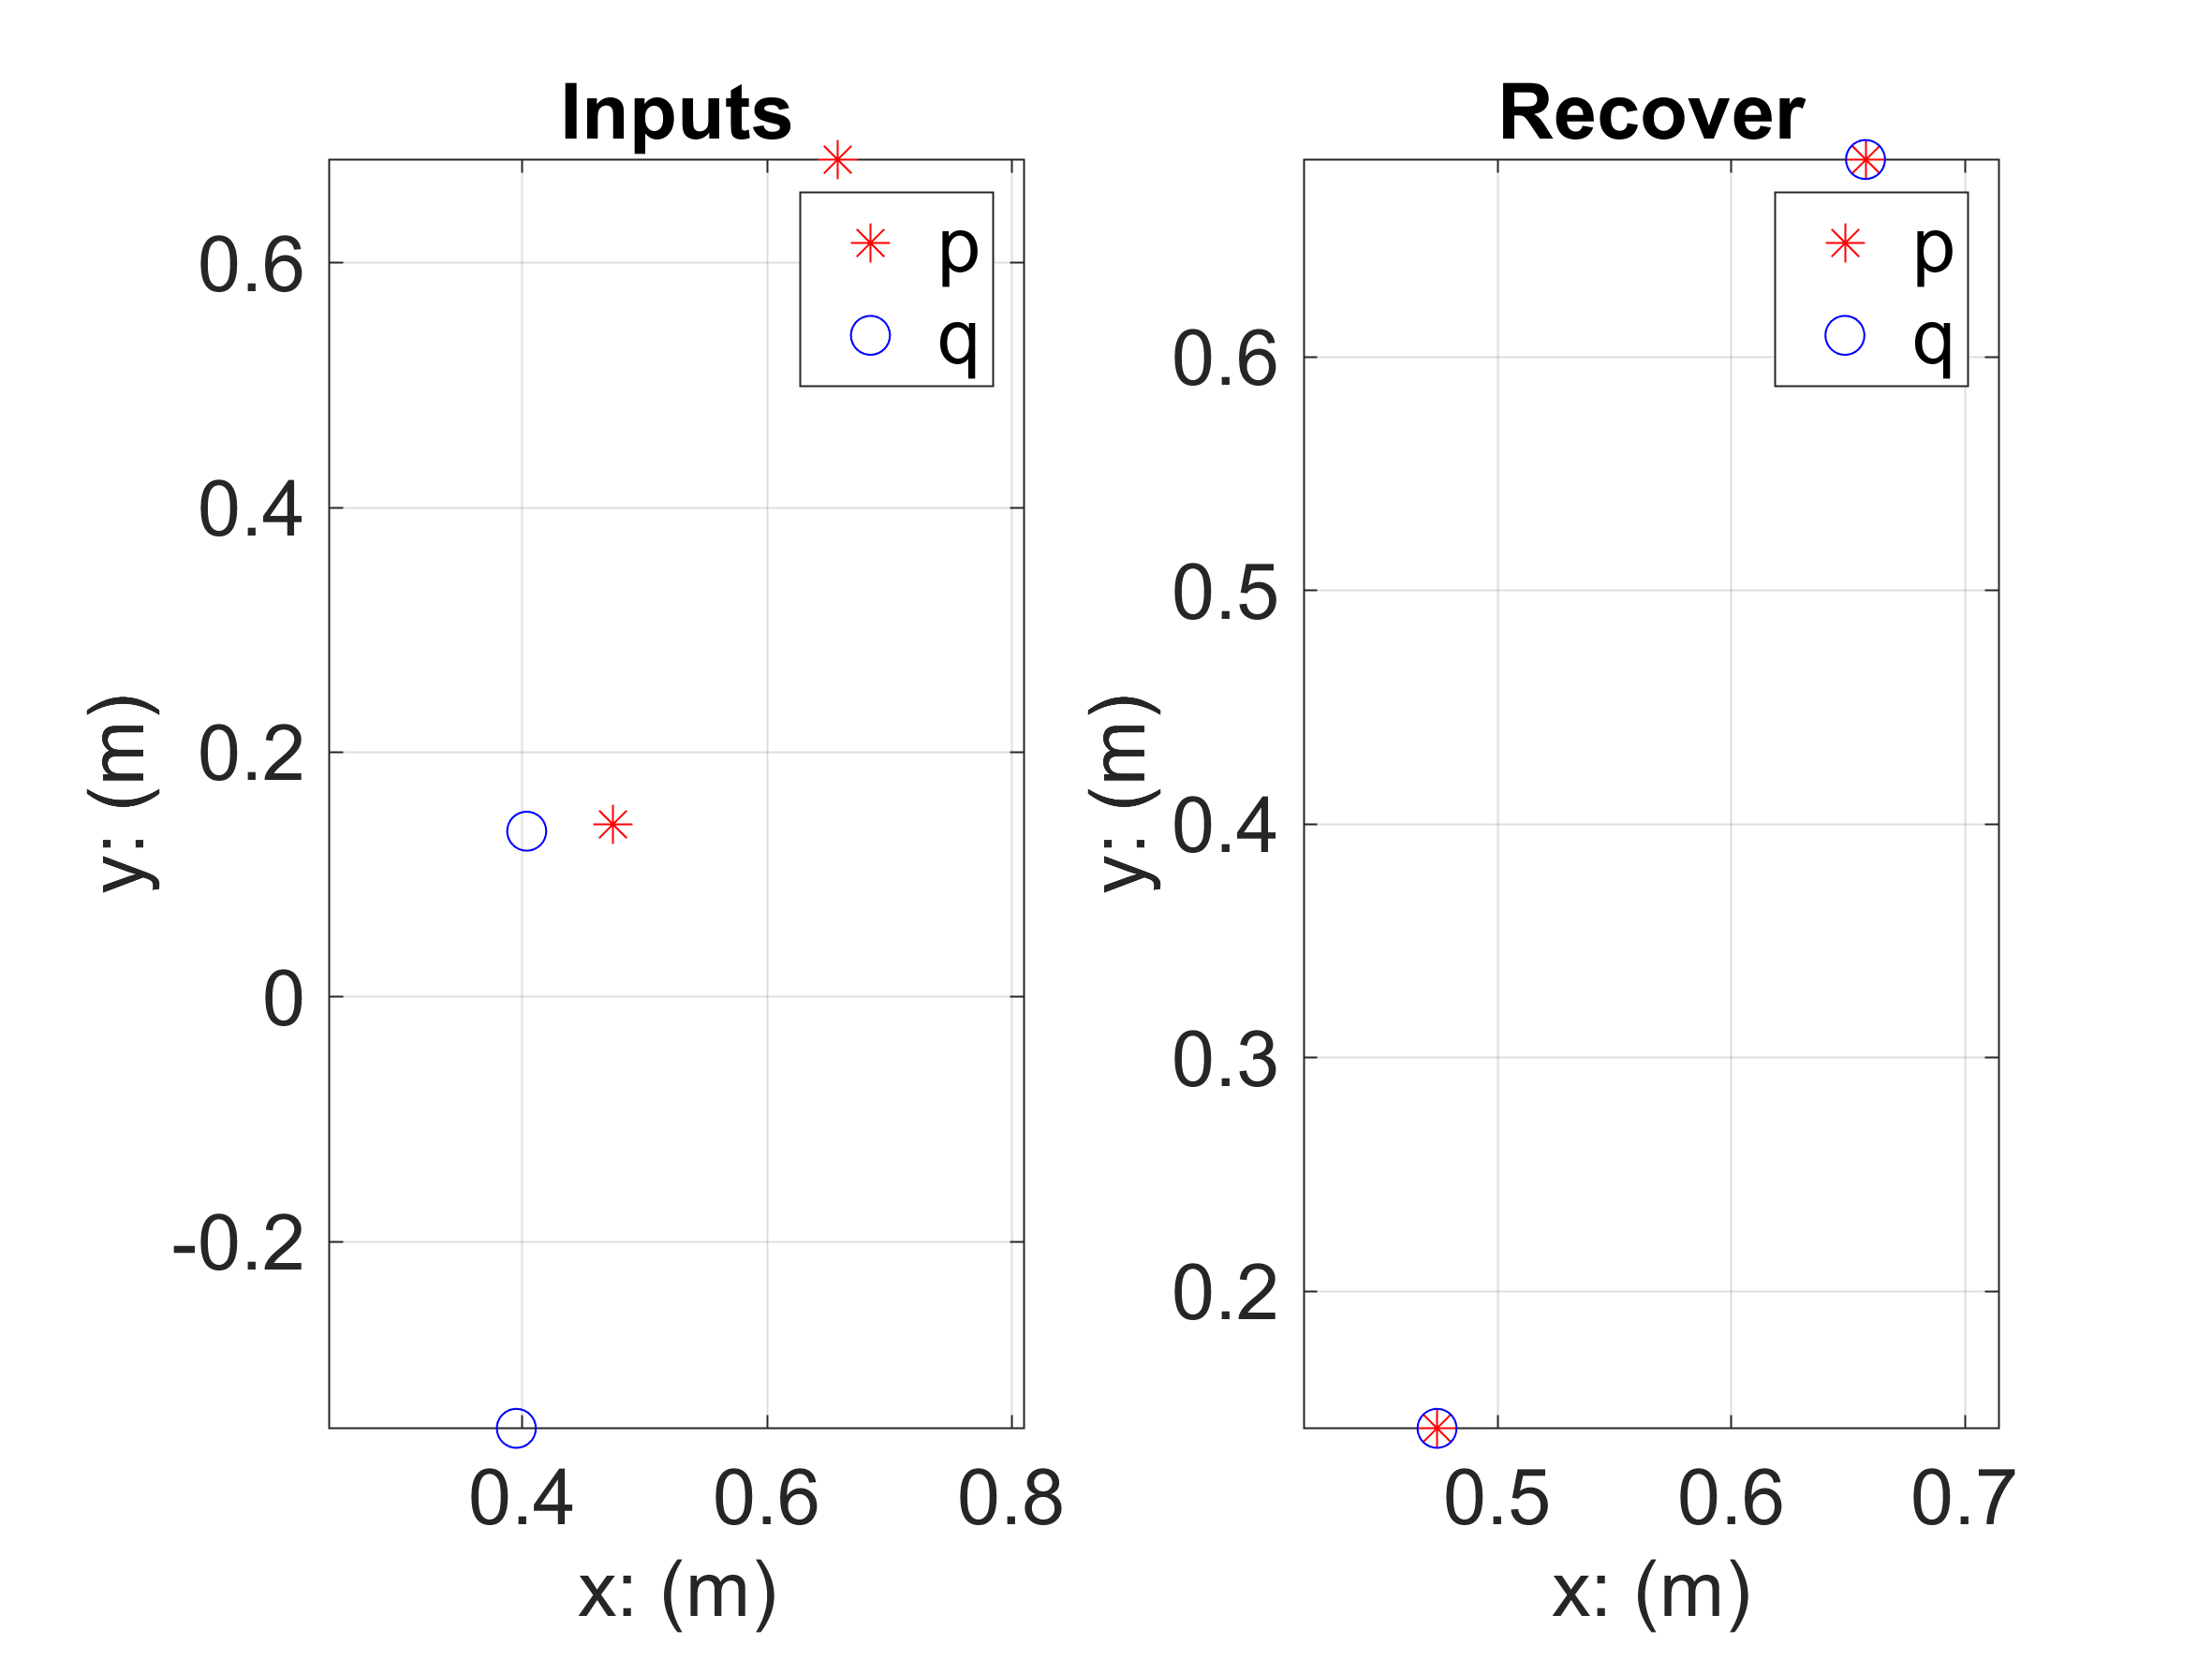
\includegraphics[width=1.0\textwidth]{figures/ex31.png} 
					\caption{Use $2$ points for estimation.}
					\end{figure}
			\end{minipage}
			\begin{minipage}{.49\textwidth}
					\begin{figure}
					\centering
					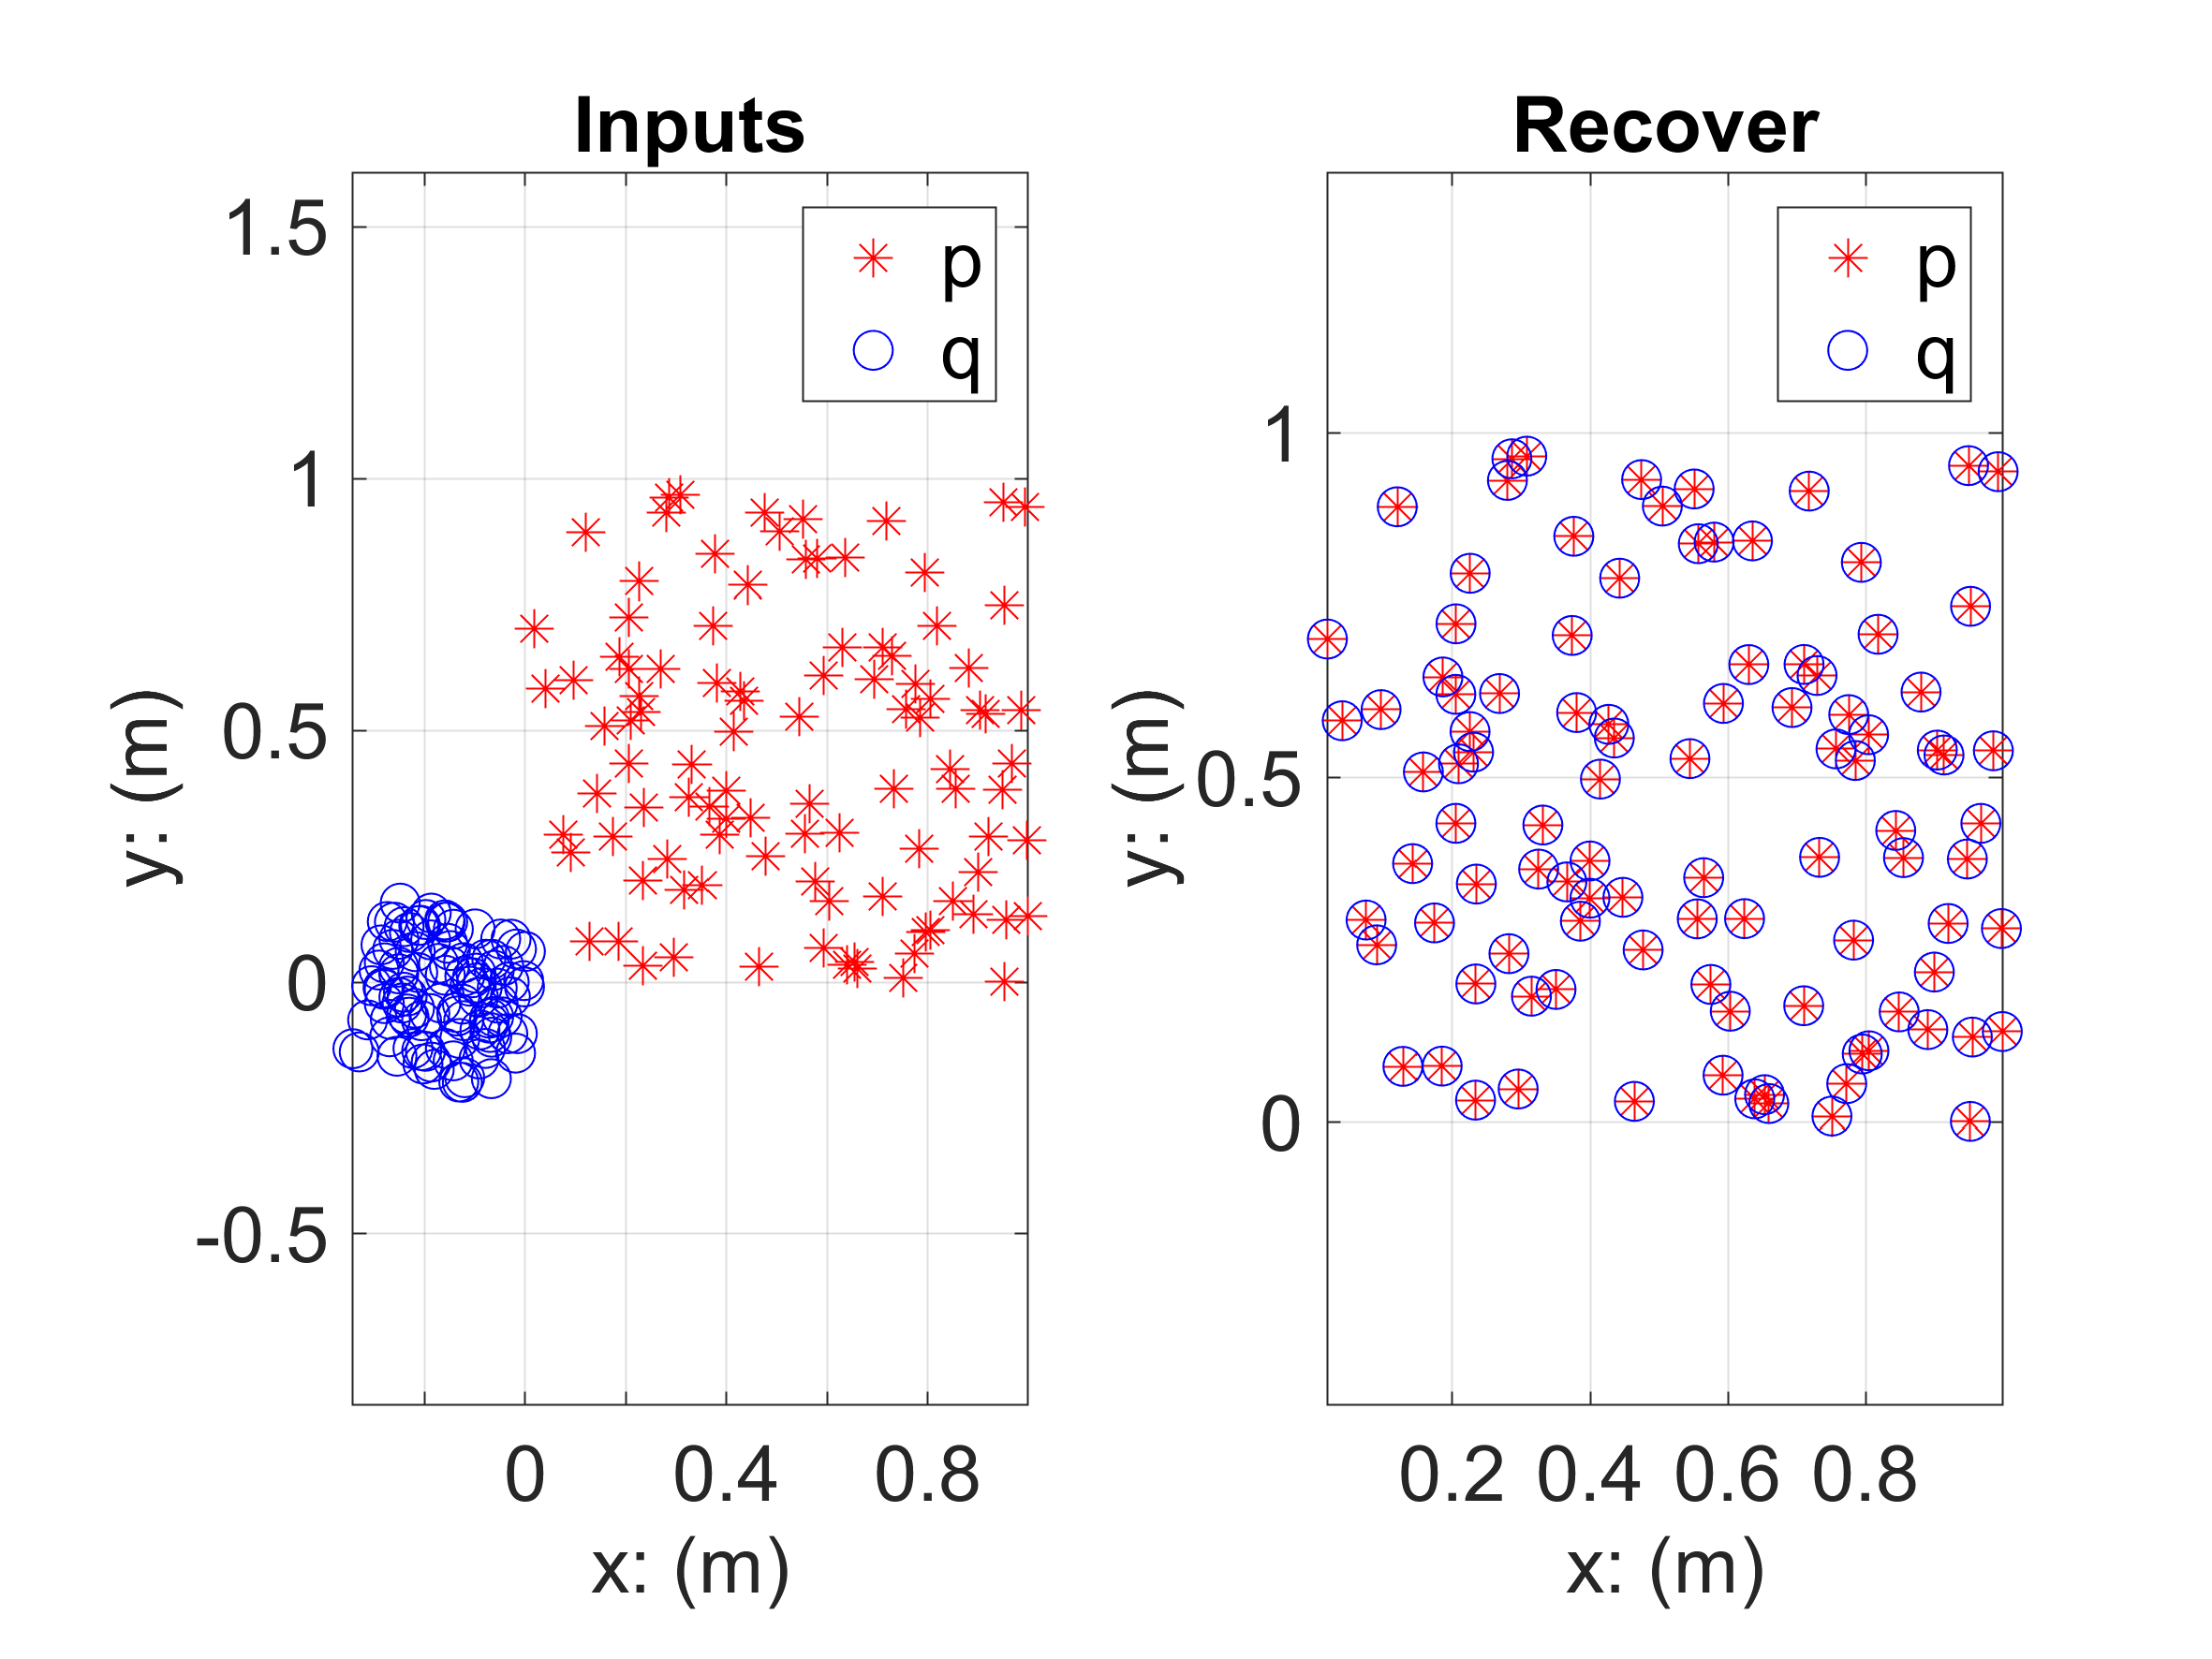
\includegraphics[width=1.0\textwidth]{figures/ex32.png} 
					\caption{Use $100$ points for estimation.}
					\end{figure}
			\end{minipage}
		}	
	\frame{
		\frametitle{SIFT matching}
			\begin{minipage}{.49\textwidth}
					\begin{figure}
					\centering
					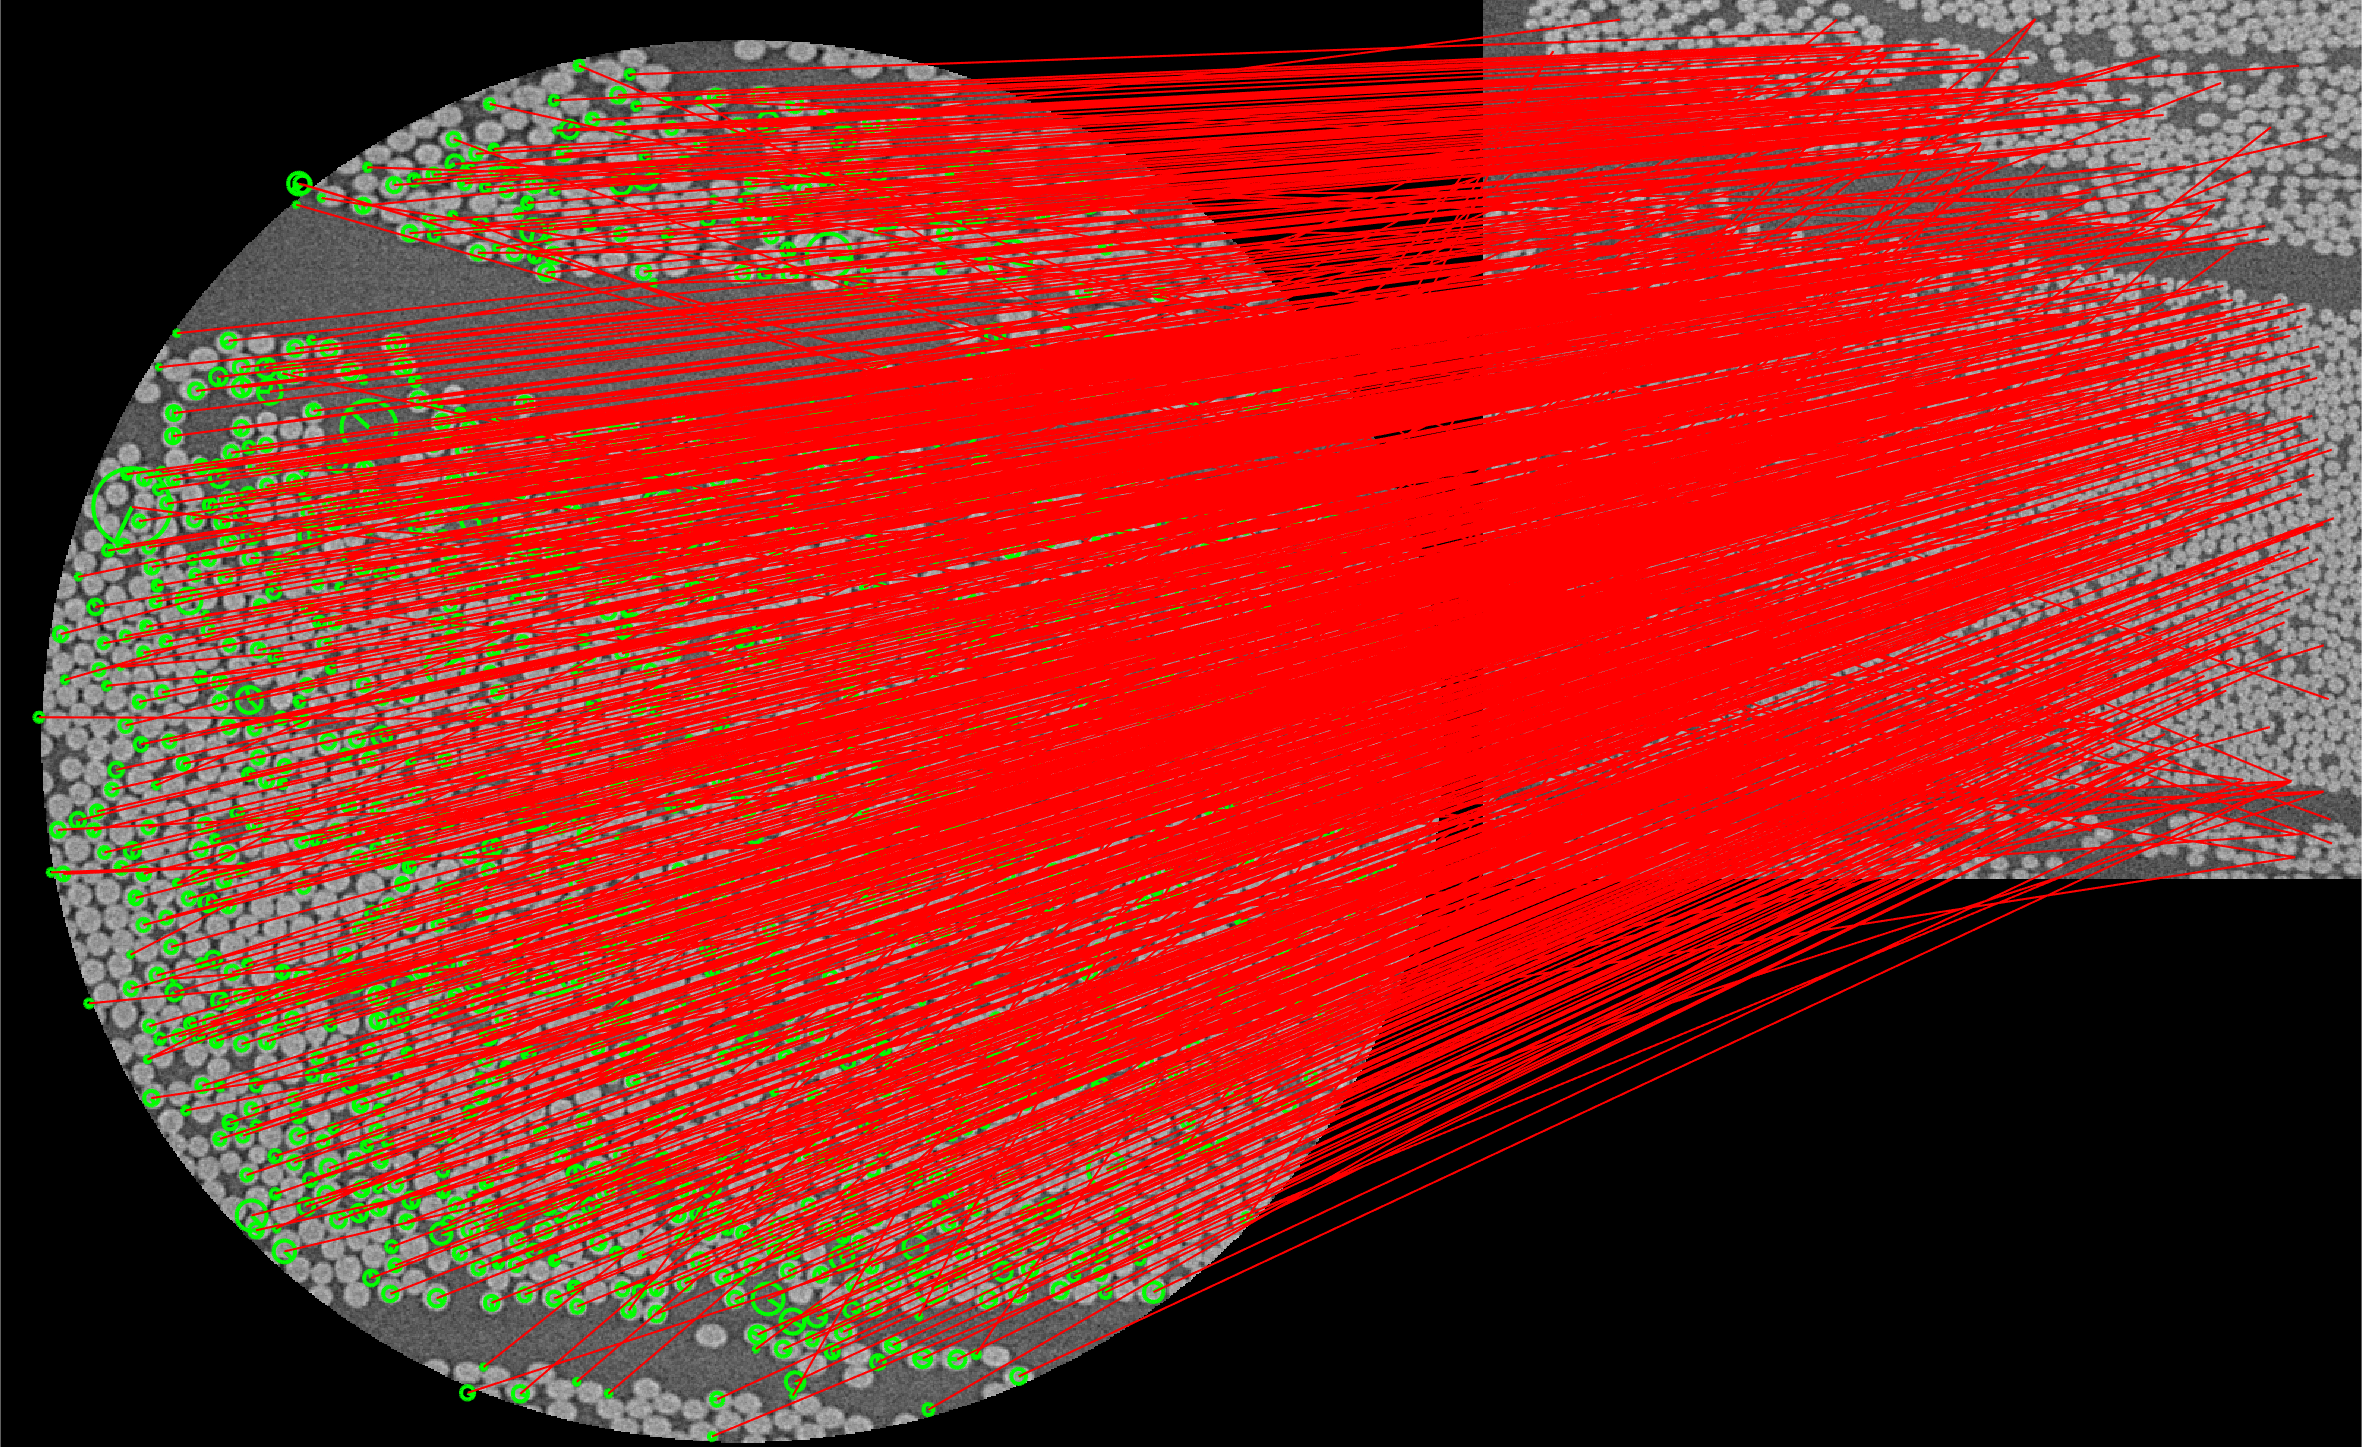
\includegraphics[width=1.0\textwidth]{figures/ex33.png} 
					\caption{Original matching result: the ratio of the best matched score and the second best matched score must be lower than $0.6$.}
					\end{figure}
			\end{minipage}
			\begin{minipage}{.49\textwidth}
					\begin{figure}
					\centering
					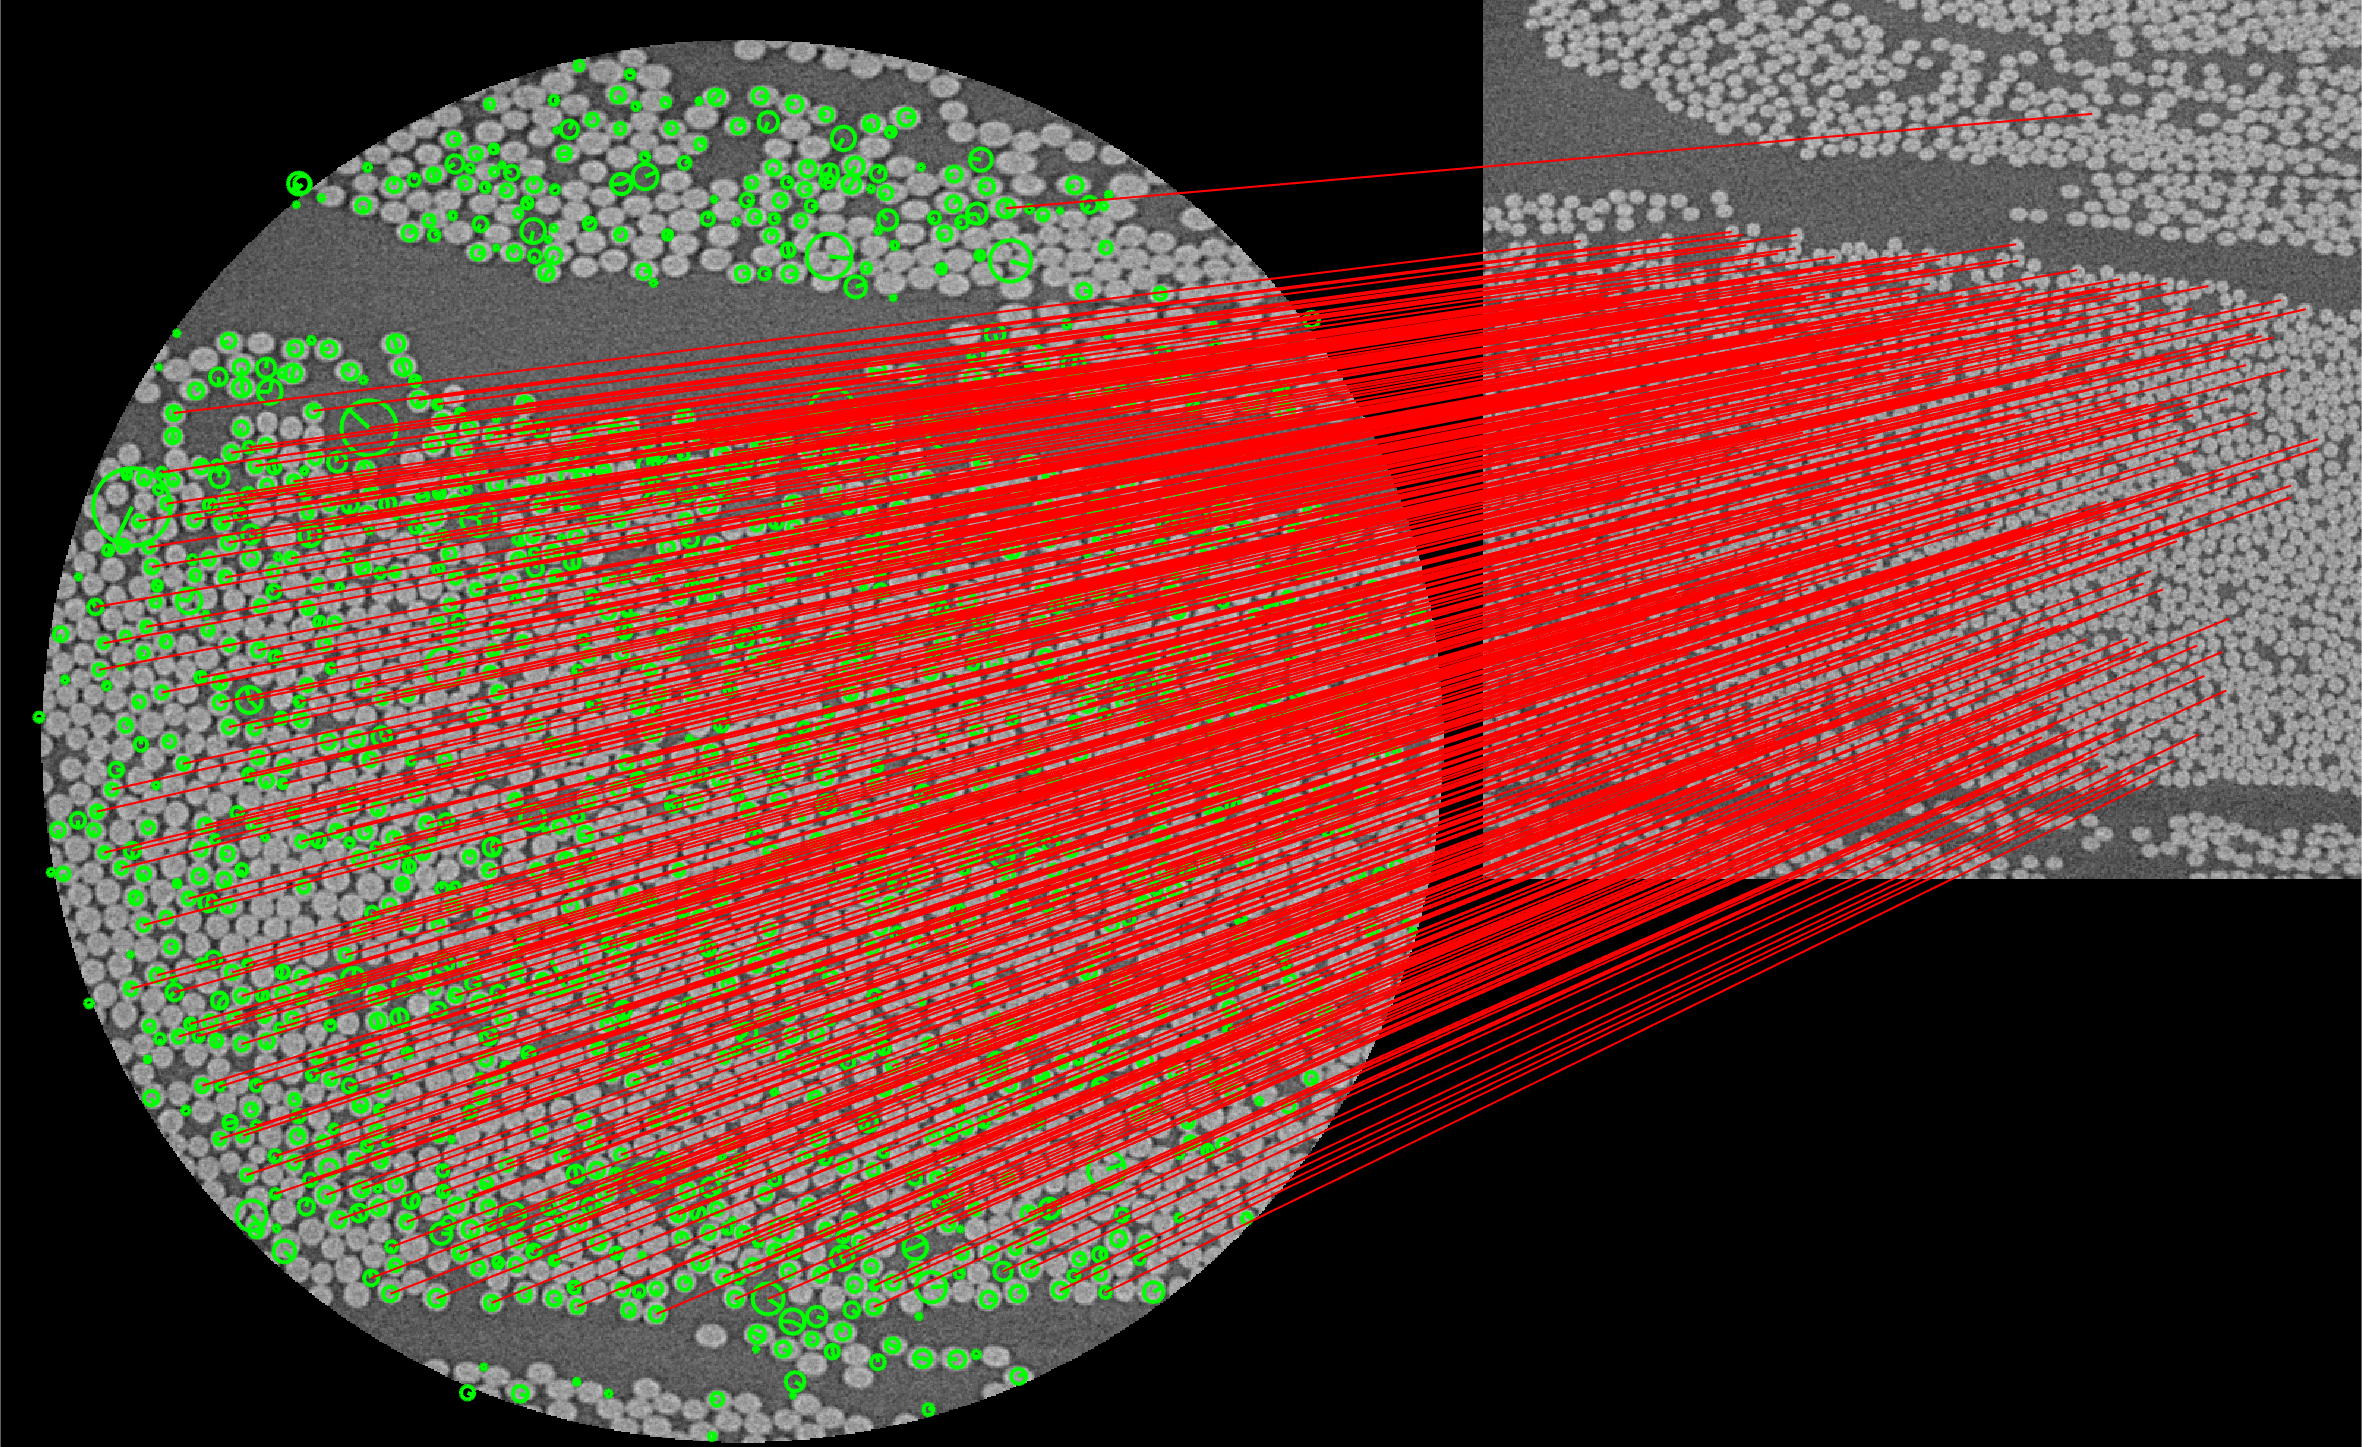
\includegraphics[width=1.0\textwidth]{figures/ex34.png} 
					\caption{Refined matching result using RANSAC: inliers are identified by applying $2$D transformation and checking the aligned distance.}
					\end{figure}
			\end{minipage}
		}	
	\frame{
		\frametitle{SIFT matching}
			\begin{minipage}{.9\textwidth}
					\begin{figure}
					\centering
					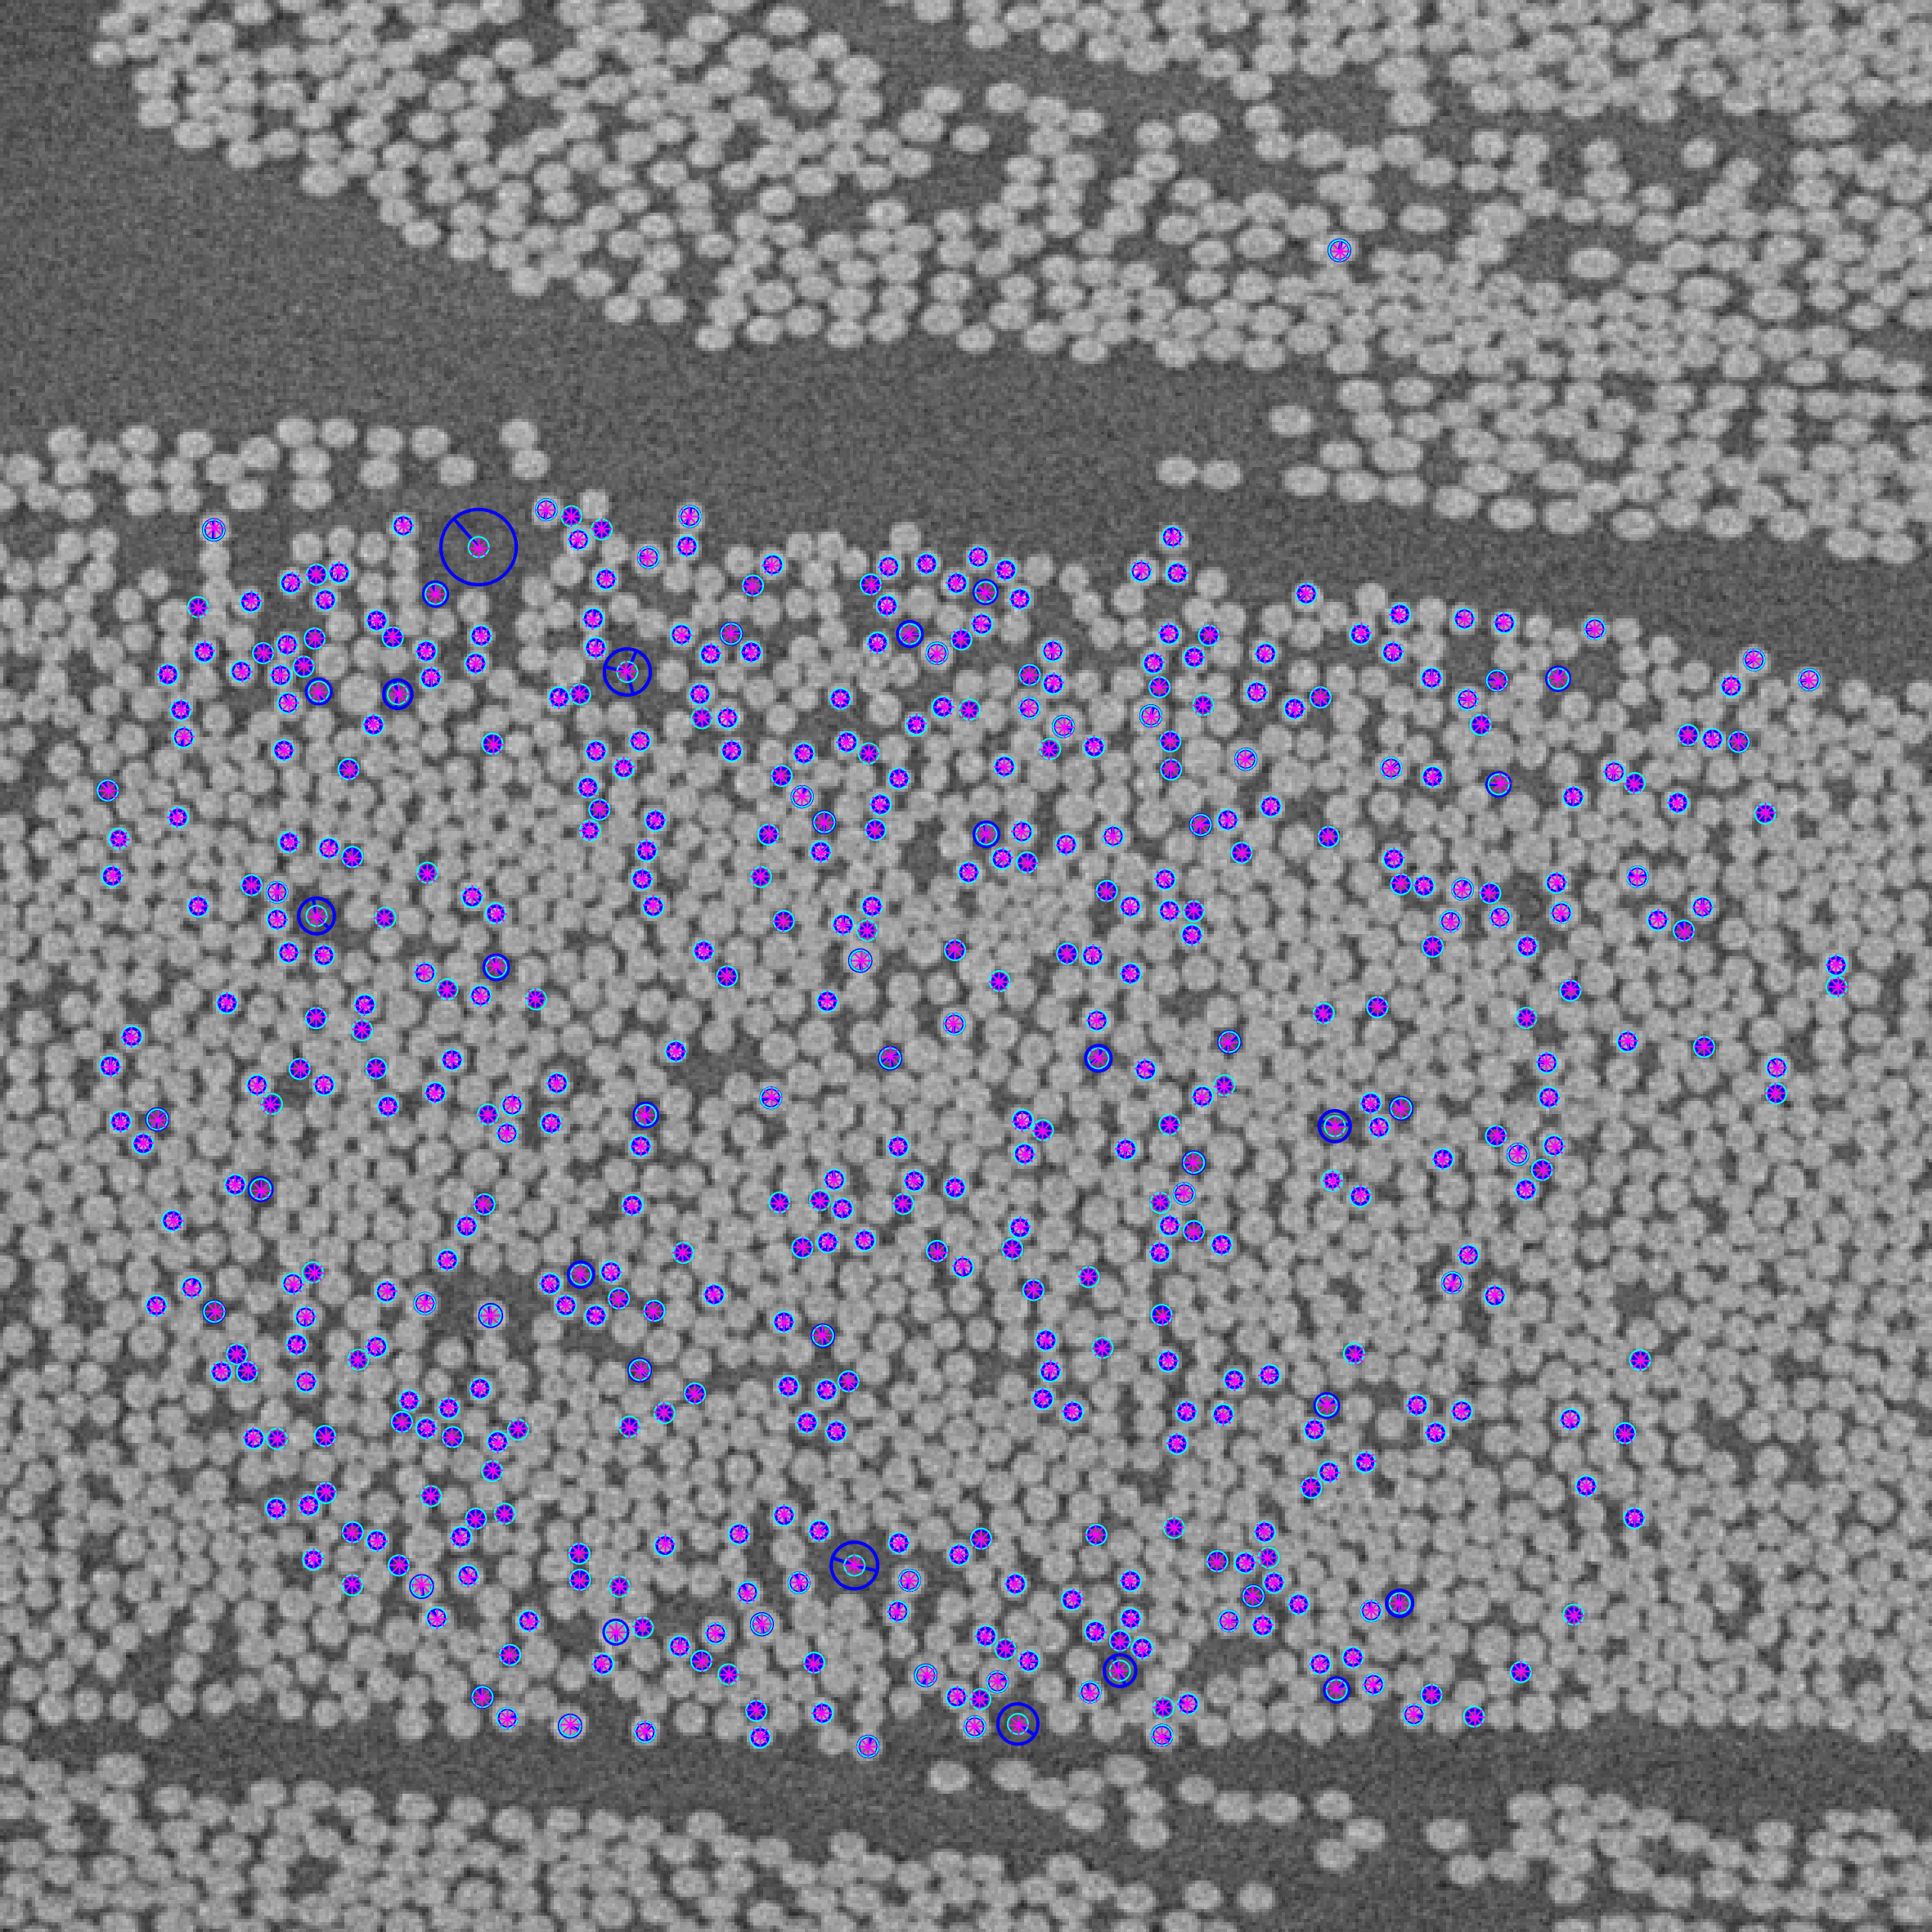
\includegraphics[width=0.45\textwidth]{figures/ex35.png} 
					\caption{Alignment of inlier features.}
					\end{figure}
			\end{minipage}
		}	
		
	\frame{
		\frametitle{Feature Based Analysis}
			\begin{minipage}{.49\textwidth}
			\begin{figure}
				\centering
				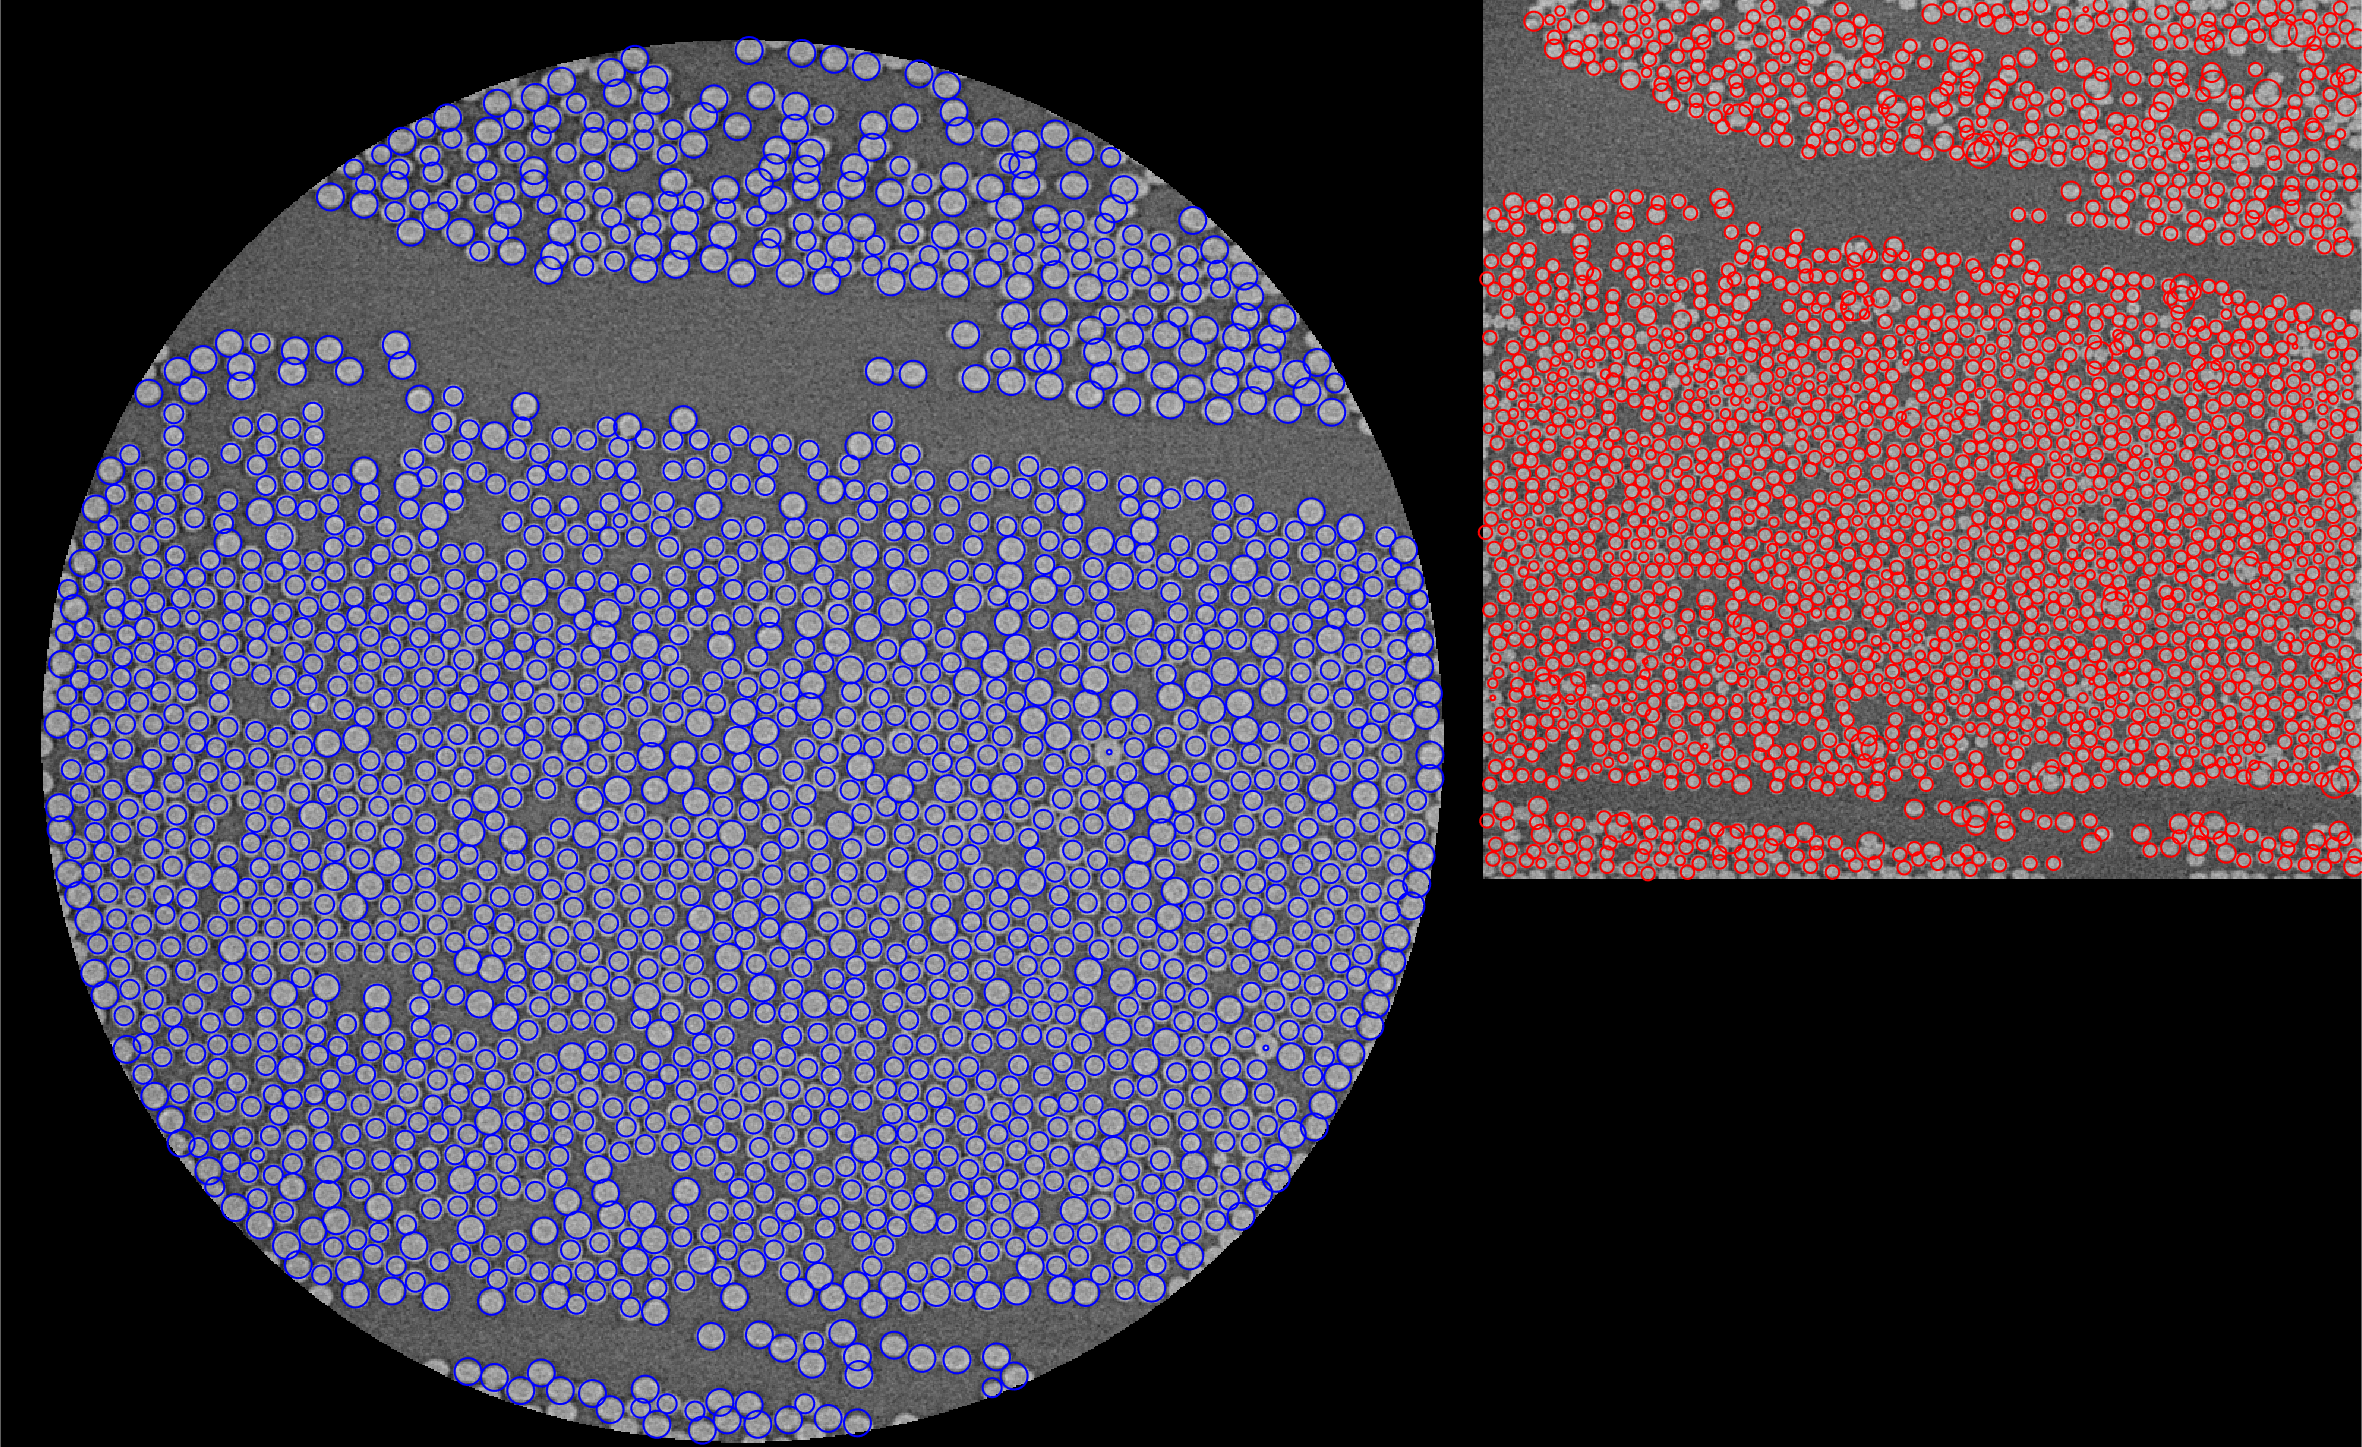
\includegraphics[width=1\textwidth]{figures/ex36.png} 
				\caption{Separate blob detection results of \textit{CT\_lab\_high\_res.png} and \textit{CT\_lab\_med\_res.png}.}
			\end{figure}
			\end{minipage}
			\begin{minipage}{.49\textwidth}
			\begin{figure}
				\centering
				\includegraphics[width=0.8\textwidth]{figures/ex37.png} 
				\caption{Aligned blob detection results by transforming blobs detected from \textit{CT\_lab\_med\_res} to \textit{CT\_lab\_high\_res}.}
			\end{figure}
			\end{minipage}
		}			
	\frame{
		\frametitle{Feature Based Analysis}
			\begin{minipage}{.99\textwidth}
			\begin{table}
		\centering
		\caption{{Quantitative result of feature based analysis}}
		\begin{tabular}{ccc}
			\hline
			\textbf{Image} &\textbf{Mean Diameter} & \textbf{Std of Diameter}  \\ \hline
			\textbf{CT\_lab\_high\_res} & $7.1153$ &   $1.1574$   \\ \hline
			\textbf{CT\_lab\_med\_res} & $7.2921$ &   $1.5451$  \\ \hline             
			\hline
		\end{tabular}
		\label{tb:mittest}
	\end{table}
	\end{minipage}
	}
	\frame{
		\frametitle{Feature Based Analysis}
			\begin{minipage}{.99\textwidth}
			\begin{figure}
				\centering
				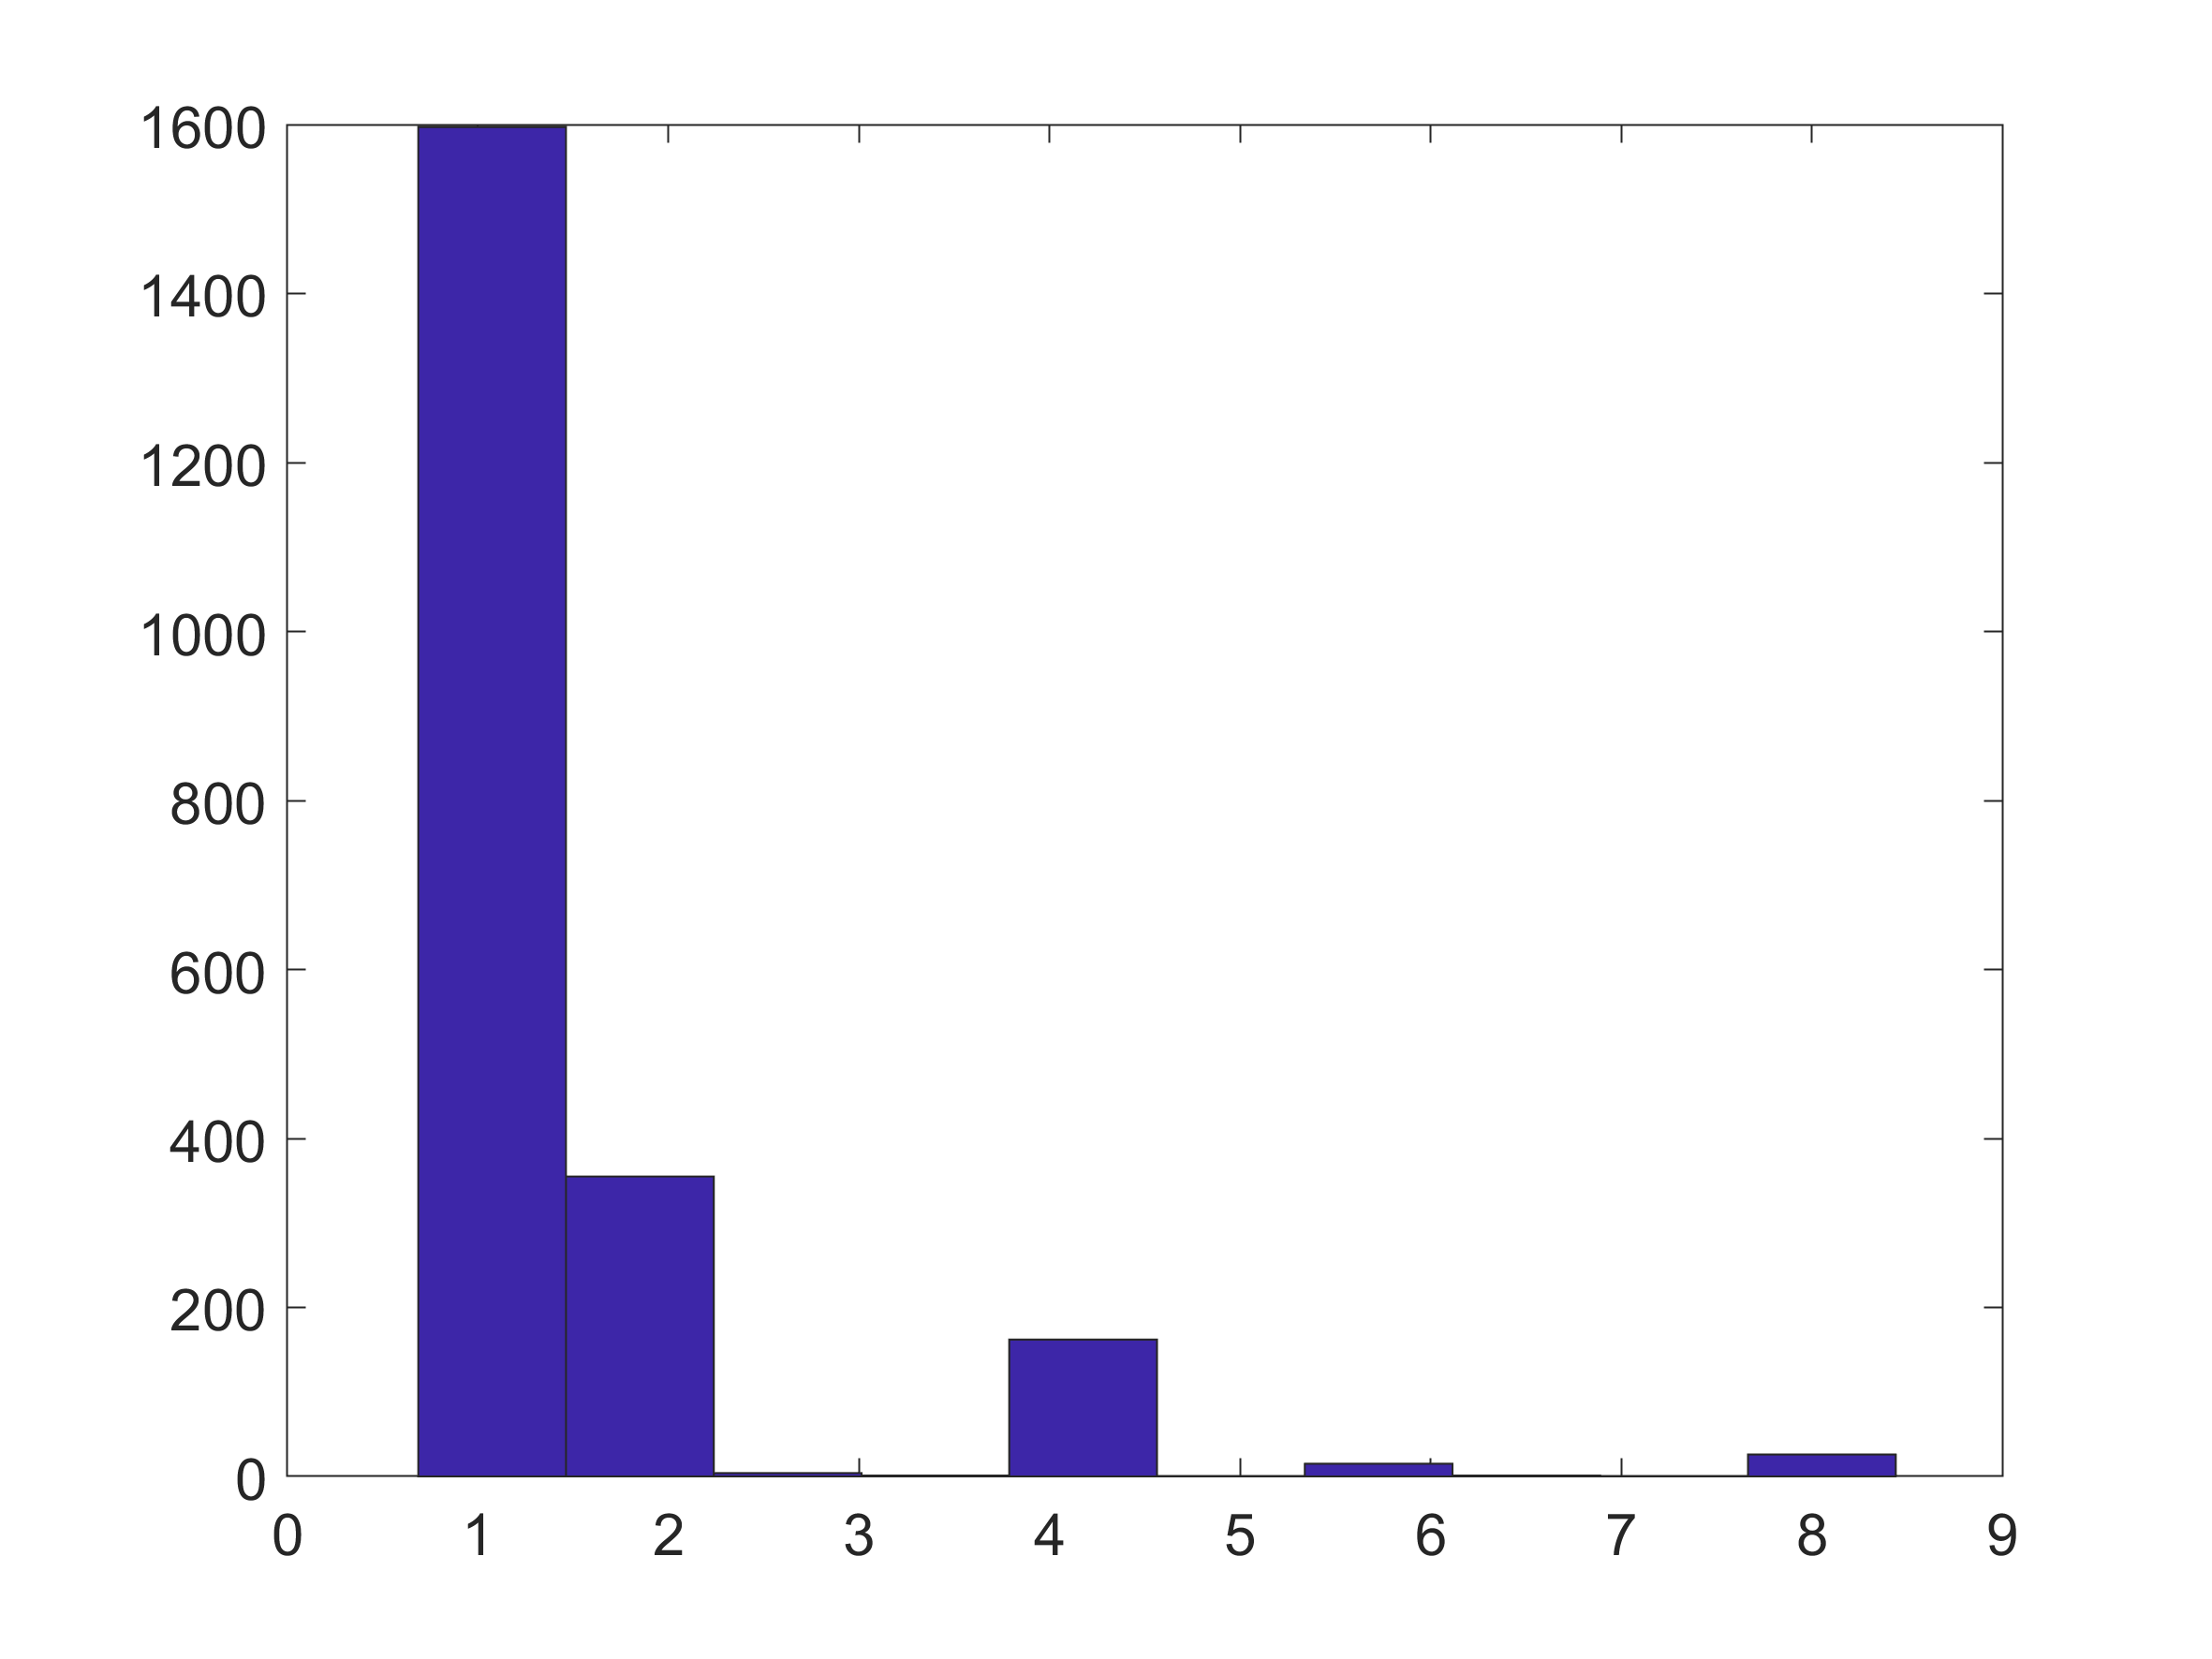
\includegraphics[width=0.5\textwidth]{figures/ex38.png} 
				\caption{Histogram of absolute difference of diameters detected in \textbf{CT\_lab\_high\_res.png} and \textbf{CT\_lab\_med\_res.png}.}
			\end{figure}
			\end{minipage}
		}			
		
	\begin{thebibliography}{00}
	\end{thebibliography}	
	
\end{document}